\documentclass[english,a4paper,11pt, oneside]{memoir}

\usepackage{amsmath}
\usepackage{lipsum}
\newtheorem{lemma}{Lemma}

% ting til memoir
\setlrmarginsandblock{3.7cm}{*}{1}
\setulmarginsandblock{3cm}{*}{1}
\setheadfoot{2\onelineskip}{\footskip}
\checkandfixthelayout

% gør at subsections også nummeres
\setsecnumdepth{subsection}

\setcounter{tocdepth}{2}

%%%%%%
% ABSTRACT STYLE
%%%%%%
\makechapterstyle{abstract}{
  \renewcommand*{\printchaptername}{}
%  \renewcommand*{\chapnumfont}{\normalfont\sffamily\huge\bfseries}
  \renewcommand*{\printchapternum}{
    \flushleft
    \begin{tikzpicture}
      \draw[fill,color=black] (0,0) rectangle (2cm,2cm);
      \draw[color=white] (1cm,1cm) node { \chapnumfont\thechapter };
    \end{tikzpicture}
  }
 % \renewcommand*{\chaptitlefont}{\normalfont\sffamily\Huge\bfseries}
  \renewcommand*{\printchaptertitle}[1]{\center\chaptitlefont\Large##1}
}
%%%%%%

%%%%%%
% PAGESTYLE
%%%%%%
\makepagestyle{main}
\makepsmarks{main}{
  \createmark{chapter}      {both}{shownumber}{}{. \ }
  \createmark{section}      {both}{shownumber}{}{. \ }
  %\createmark{subsection}   {both}{shownumber}{}{. \ }
  % \createplainmark{toc}     {both}{\contentsname}
  % \createplainmark{lof}     {both}{\listfigurename}
  % \createplainmark{lot}     {both}{\listtablename}
  % \createplainmark{bib}     {both}{\bibname}
  % \createplainmark{index}   {both}{\indexname}
  % \createplainmark{glossary}{both}{\glossaryname}
}
\makeoddhead{main}{}{}{\rightmark}
\makeevenhead{main}{\leftmark}{}{}
% sidens fod: sidetal
\makeoddfoot{main}{}{}{\thepage}
\makeevenfoot{main}{\thepage}{}{}
% smid en linie under
\makeheadrule{main}{\textwidth}{\normalrulethickness}

% \setsecheadstyle{\large\bfseries\raggedright}
% \setsubsecheadstyle{\normalsize\bfseries\raggedright}

\nouppercaseheads
\pagestyle{main}
%%%%%%

%%%%%%
% CHAPTER PAGE STYLE
%%%%%%
% \makeoddhead{plain}{}{}{}
% \makeevenhead{plain}{}{}{}
% % sidens fod: sidetal
% \makeoddfoot{plain}{}{}{\thepage}
% \makeevenfoot{plain}{\thepage}{}{}
% \aliaspagestyle{chapter}{plain} % make chapter pages same page style as everything else


%%%%%%
% CHAPTER STYLE
%%%%%%
\usepackage{tikz}

\makechapterstyle{box}{
  \renewcommand*{\printchaptername}{}
%  \renewcommand*{\chapnumfont}{\normalfont\sffamily\huge\bfseries}
  \renewcommand*{\printchapternum}{
    \flushleft
    \begin{tikzpicture}
      \draw[fill,color=black] (0,0) rectangle (2cm,2cm);
      \draw[color=white] (1cm,1cm) node { \chapnumfont\thechapter };
    \end{tikzpicture}
  }
 % \renewcommand*{\chaptitlefont}{\normalfont\sffamily\Huge\bfseries}
  \renewcommand*{\printchaptertitle}[1]{\flushleft\chaptitlefont##1}
}
%%%%%%


% used for flow charts
\usetikzlibrary{shapes,arrows}
% Define block styles
\tikzstyle{decision} = [diamond, draw, fill=blue!10,
    text width=9em, text badly centered, node distance=3cm, inner sep=0pt]
\tikzstyle{block} = [rectangle, draw, fill=blue!10,
    text width=10em, text centered, rounded corners, minimum height=4em]
\tikzstyle{line} = [draw, -latex']

\usepackage{afterpage}
\usepackage[utf8]{inputenc}	%Tillader danske tegn
\usepackage[T1]{fontenc}	%Tillader danske tegn
\usepackage{graphicx}		%Tillader indsættelse af billeder
\usepackage{dcolumn}		%Bruges til at lave matematiske tabelsøjler... se datatabel
\usepackage{mathtools}		%Ekstra matematik... bare lad den være, du får muligvis brug for den.
\usepackage{float}
\usepackage[locale=DE, range-phrase=--, range-units=single, group-separator={ }]{siunitx}
\sisetup{output-decimal-marker = {.},separate-uncertainty=false,fraction=nice,fraction-function=\tfrac,alsoload=binary,obeyall}
%\sisetup{output-decimal-marker = {.}}
\usepackage{microtype}
\usepackage{amssymb}
\usepackage{rotating}
\usepackage[round]{natbib}
\usepackage{booktabs}
\setlength{\heavyrulewidth}{0.15em}
\setlength{\lightrulewidth}{0.08em}

% Where to look for figures
\graphicspath{ {./figures/} }

\newcommand{\mc}[1]{\multicolumn{1}{c}{#1}}
%\usepackage{threeparttable}
%\usepackage{multirow}

\numberwithin{equation}{chapter}
\numberwithin{table}{chapter}
\numberwithin{figure}{chapter}
\usepackage{varioref}
\usepackage[colorlinks=true,citecolor=blue,linkcolor=black]{hyperref}
\usepackage[draft]{fixme}
\linespread{1.05}
\usepackage[sc]{mathpazo}
\usepackage{wasysym}
\usepackage{cite}
\usepackage{multirow}
\usepackage{subcaption}
%\newsubfloat{figure}
%\RequirePackage[caption=false,position=top]{subfig}
%\let\subtop\subfloat

\usepackage{caption}
\captionsetup[figure]{labelfont=bf, textfont={}}
\captionsetup[table]{labelfont=bf, textfont={}}

\parindent 0pt
\setlength{\parskip}{2mm plus0mm minus0mm}

% Included chapters
\includeonly{
introduction,
Background,
Development,
Results,
Discussion,
conclusion
}


% Macros
\newcommand{\sref}[1]{Section~\ref{#1}}
\renewcommand{\fref}[1]{Figure~\ref{#1}}
\renewcommand{\tref}[1]{Table~\ref{#1}}
\renewcommand{\eqref}[1]{Equation~(\ref{#1})}
\renewcommand{\vec}[1]{\mathbf{#1}}
\newcommand{\half}[0]{\frac{1}{2}}
\newcommand{\mean}[1]{\ensuremath{\left\langle #1 \right\rangle}}
\newcommand{\pdiff}[2]{\frac{\partial #1}{\partial #2}} % Partial derivative
\newcommand{\ppdiff}[2]{\frac{\partial^2 #1}{\partial #2^2}} % Partial derivative
\newcommand{\mat}[1]{\ensuremath{\boldsymbol{#1}}}
\newcommand{\norm}[1]{|#1|}
\newcommand{\cov}[0]{\text{cov}}

\usepackage{listings}
\usepackage{color}
\usepackage{textcomp}
\definecolor{listinggray}{gray}{0.9}
\definecolor{lbcolor}{rgb}{1,1,1}
\lstset{
	backgroundcolor=\color{lbcolor},
	tabsize=2,
	rulecolor=,
	language=matlab,
        basicstyle=\scriptsize,
        upquote=true,
        aboveskip={1.5\baselineskip},
        columns=fixed,
        showstringspaces=false,
        extendedchars=true,
        breaklines=true,
        prebreak = \raisebox{0ex}[0ex][0ex]{\ensuremath{\hookleftarrow}},
        frame=single,
        showtabs=false,
        showspaces=false,
        showstringspaces=false,
        identifierstyle=\ttfamily,
        keywordstyle=\color[rgb]{0,0,1},
        commentstyle=\color[rgb]{0.133,0.545,0.133},
        stringstyle=\color[rgb]{0.627,0.126,0.941},
}

%%%%% BEGIN DOCUMENT %%%%%
\begin{document}
\pagenumbering{roman}
\pagestyle{plain}
%% BOS FORSIDESKABELON

\begin{titlingpage}

\begin{center}

\vspace*{0cm}
\huge
\textsc{Experimental tests of the stability of a modular spectrograph for use in au-sat}\\
\vspace{1.5cm}


\includegraphics[width=.9\textwidth]{au_logo.png}

\vspace{1cm}

\large
{
    Steffan Johan Kirk\\
    Student number: 201303635
    ~
   
}


\vspace{1cm}

{
  Supervisor : Victoria Antoci\\
  
  ~\\
  Institute for Physics and Astronomy, Aarhus University
}

\vspace{0.5cm}
{June 2016}\\


\end{center}

%\newpage

%%%%%
% The back of the frontpage
%%%%%
%colophon

\end{titlingpage}

%\setcounter{page}{3}
\chapter*{Preface}
This bachelor thesis is the result of work done at the Department of Physics and Astronomy of Aarhus University. I owe thanks to my supervisor Victoria Antoci, for guidance on the development of the experiments and for answering my many questions and without whom this work would not be possible. Furthermore i owe thanks to Mads Fredslund for technical help and the Electronics department at the Department of Physics and Astronomy of Aarhus University for help on the circuit design in this thesis.
\chapterstyle{abstract}
\vspace{6cm}
\chapter*{Summary}
%\lipsum[1-3]
\chapterstyle{box}

In a workshop aimed at discussing the possibility of the Department for Physics and Astronomy Aarhus University, launching a nanosatellite space mission, it was decided to test a potential spectrograph to fly on the mission. In this thesis three experiments were designed to simulate the environment the satellite would be subject to in space to test the spectrograph. The stability of measurements from an of-the-shelf spectrograph was examined for stationary conditions and for simulated pointing of the satellite via vibrations. The stationary measurement showed that the spectrograph was able to measure the wavelength for six of the emission lines of Helium, with an uncertainty ranging from \SIrange{0.1d-3}{1.1d-3}{\nano\meter} and for the simulated pointing with the uncertainty in the range \SIrange{0,01}{0,54}{\nano\meter}. Furthermore the temperature variations for a satellite i orbit were simulated to examine the dependency of the temperature for measurements from the spectrograph. It was found the measured wavelength for the Helium emission lines were shifted linearly as a function of temperature, but the shifts over the wavelength range of the spectrograph were not uniform. The range of the shift in wavelength as a function of temperature was \SIrange{-0,5}{0,35}{\nano\meter}. Finally it was concluded that further testing of the spectrograph was needed to verify the results.
\newpage\thispagestyle{empty}\mbox{}%\newpage
\renewcommand{\contentsname}{Contents}
\tableofcontents*
%\newpage\thispagestyle{empty}\mbox{}\newpage
\newpage
\pagenumbering{arabic}
\setcounter{page}{1}
\pagestyle{main}

%%%%% INCLUDE CONTENT FILES %%%%%

%\include{filename}

\chapter{Introduction}

The motivation for this bachelor thesis arose from the \emph{AU-SAT Workshop} meeting that took place in late November 2015. The workshop discussed the possibility of the Department of Physics and Astronomy of Aarhus University building a small satellite named the AU-SAT. 

The AU-SAT should make use of new technology to allow for a design much smaller than traditional satellites in space, making the mission affordable for Aarhus University. The satellite would be build in partnership with the Danish small satellite company \emph{GomSpace}.

The idea for a small satellite mission designed by the Department of Physics and Astronomy of Aarhus University, was inspired by two earlier small satellite missions, MOST and BRITE, designed by the Space Flight Laboratory and the Institute for Aerospace Studies at the University of Toronto respectively. These previous missions had shown that science could be preformed with observations made from micro- and nano-satellites.
\\
\\
The AU-SAT mission, however, is not meant to be a copy of the MOST and BRITE missions. AU-SAT will have to be able to preform observations that are not possible from any other small satellite mission. BRITE and MOST are photometric missions, whereas AU-SAT would spectroscopic. The AU-SAT would be a satellite using a spectrograph with a wide wavelength range, and still be able to fit inside a shoe box.
The possible missions for the AU-SAT include,

\begin{itemize}
\item UV spectrum observations of stars.
\item Observations of newly discovered eclipsing binary stars by NASA's TESS mission, allowing the Institute of Physics and Astronomy of Aarhus University to be on the front line for new discoveries.
\item Observations of stellar pulsations, allowing for a better understanding of the interiors of stars. AU-SAT would be the first to use a spectrograph capable of making these observations over such a broad band. 
\item Observe exo-planet candidates discovered by TESS, making discoveries of new exo-planets possible.
\end{itemize}

The conclusion of the AU-SAT workshop was to continue examining the possibility for creating the AU-SAT mission and start testing a possible small spectrograph, for use onboard the AU-SAT, with which this thesis is concerned. 


\chapter{Background}
\section{Observations In Space}
Observations of objects in space can be conducted both from Earth and from orbits in space.
\citet{Mons} talks about how performing astronomy from Earth is limited by the filtering and distortion of electromagnetic radiation by the Earth's atmosphere, a feature that protects life on Earth from ultraviolet rays, x-rays and gamma rays. The altitude needed to detect the different bands of the electromagnetic spectrum is illustrated in Fig. \ref{fig: em_surface}. From Earth radio waves, near-infrared and visible light are observable. For observing other frequencies of the electromagnetic spectrum it is necessary to have observatories in space where the atmosphere is not present. There are several ways of observing and examining objects in space. To make observations from space most often the equipment needed is launched  into space on board a satellite and the two most commonly used methods for examining astronomy objects in space are via \emph{Photometry} and \emph{Spectroscopy.}

\afterpage{
\begin{figure}[h]
\centering
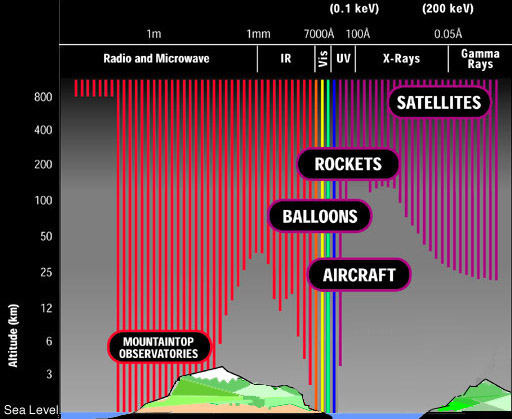
\includegraphics[width=.6\textwidth]{em_earth}
\caption[hej]{Illustration of the altitude needed to observe the different bands of the electromagnetic spectrum. Fig. from (Online).\footnotemark}
\label{fig: em_surface}
\end{figure}
\footnotetext{\url{http://migall.fastmail.fm.user.fm/astronomy/telescopes_detectors/emr/page6.htm}}
}

\section{The Space Mission Life Cycle and Architecture}
When planning a mission in space, a great amount of planning must first be done back on Earth. This is the case whether planning a manned mission or launching a satellite into orbit.
\citet{smad} gives a nice overview of the progress of designing a space mission:

\begin{itemize}
\item \emph{Concept exploration}, The initial study phase, in which a broad definition of the space mission and its components.

\item \emph{Detailed development}, the formal design phase, which results in a detailed definition of the system components and test of hardware and development.

\item \emph{Production and deployment}, the construction of the ground and flight hardware and launch of the final system. 

\item \emph{Operations and support}, the day-to-day operations of the space system, its maintenance and support, and its deorbit or recovery at the end of the mission life. 
\end{itemize}

Furthermore all space missions consist of a set of elements and the arrangement of these elements form the space mission architecture \citep{smad}.

The \textit{subject} of the mission is the object to be examined that either interacts with or is measured by the \textit{payload}.
\\

The \textit{payload} consist of the hardware and software that measure or interact with the subject. The payload is contained within the \textit{platform} which also holds all the subsystems that handle, altitude, orbit, power, telemetry and data. The \textit{payload} and \textit{platform} are together called the \textit{spacecraft}. The \textit{spacecraft} for the AU-SAT mission would be the satellite with a telescope, an onboard computer, for communications and onboard data processing and likely a spectrograph to analyze the incoming light from the stars. 
\\

The \textit{launch system} includes the launch facility and the launch vehicle that is needed to launch the payload into orbit. 
\\

The \textit{orbit} is the path or trajectory of the spacecraft. There are several orbits the spacecraft enters before it reaches its mission orbit. An often used orbit is the \textit{low earth orbit} with an altitude between 200-2000 \si{\kilo\meter}. Most satellites in orbit use the \textit{low earth orbit}, which is also used by the \textit{International Space Station} which houses the astronauts in space. 
\\

The \emph{ground systems} consist of the ground stations that connect with the spacecraft, so the operators are able to control the spacecraft and receive the 	telemetry and the mission data. 
\\

For the AU-SAT the Institute of Physics and Astronomy Aarhus University will decide the subject of the mission and determine the payload for the satellite. The scope of this bachelor's thesis is to examine the stability of the spectrograph that could be included in the payload if the satellite is launched. The spacecraft bus will be delivered by the Danish Cubesat company GomSpace. For the launch system, it will be required to buy a free spot on a commercial rocket, that would deliver the spacecraft on a desired orbit for observations. 

\section{Nanosatellites - Cubesats}
\label{satellite}
In the last decade launching a satellite into space has become more accessible with the introduction of smaller and cheaper nanosatellites, also called Cubesats. A Cubesat is small satellite made up of multiples of \num{10 x 10 x 10} \si{\centi\meter} cubic units. Cubesats are often build with off the shelf components for their electronics	 and structure. Only in recent time the technology has evolved to allow for high performance miniature star trackers, that are used to determine the orientation of the satellite in space. With a star tracker and a pointing controller, consisting of three axis reaction wheels used to rotate the satellite, the satellite is able to keep its needed orientation for observations in space \citep{brite}. As a satellite orbits around Earth it needs to rotate in order to keep pointing at the object being observed if observations are made over a long period of time. The continuous movement from the pointing of the satellite results in a change of how the light hits the light entrance of the satellite. Shown in Fig. \ref{fig: pointing} is a simulation for the BRITE telescope, of how a star being observed moves over the light entrance as a result of the pointing of the satellite. 
Satellites in orbit are also subject to temperature variations due to the satellite being exposed to direct sunlight or being in the shadow of the Earth. If build the AU-SAT will consist of six cubic units and will be tested to verify if can hold up to the environment in space.

\begin{figure}[h]
\centering
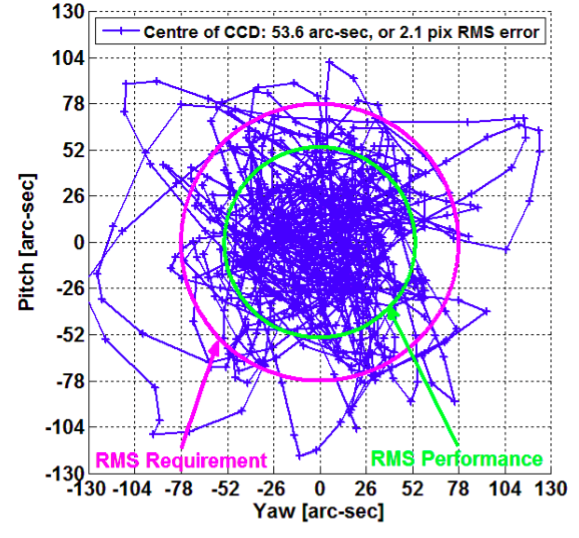
\includegraphics[width=.5\linewidth]{pointing.png}
\caption[]{Simulation of the movement over the light entrance of an object being observed from pointing of satellite. Fig. from \citep{brite}.}
\label{fig: pointing}
\end{figure}

\section{Photometry}
Photometry is concerned with measuring the change in intensity of an astronomical object's electromagnetic radiation. In its most basic form, photometry is conducted by gathering light through a telescope on to a photosensitive instrument which records the light energy, coming from the object being examined. Photometry is often performed within a selected wavelength range by adding filters to the telescope that allow the wanted wavelength to pass through. Photometry, for example, can be used to measure oscillations in stars by monitoring the brightness and colour fluctuations over time \citep{Mons}. Some of the current space missions that use photometry include MONS, BRITE and The Kepler Space Telescope.

\section{Spectroscopy}
Spectroscopy uses an instrument called a spectrograph, that separates light into a frequency or wavelength spectrum and records the signal using a camera. Most often the deflection of the light is produced either by refraction or by diffraction. The deflection of light by refraction uses that light of different wavelength is spread in different angles when traveling from one medium to another medium with a different refractive index. Deflection of light by diffraction makes use of the phenomena which occurs when a wave encounters an obstacle. Diffraction is defined as the bending of light around the corners of a obstacle. To split light into several beams traveling in different directions a diffraction grating can be used. A diffraction grating is an optical component with a periodic structure typically of ridges on their surface. The deflection of the light hitting the grating depends on the spacing of the grating and the wavelength of the light. The light is then focused on to a detector, often a CCD detector is used. The CCD detector consists of an array of pixels that measure the intensity of the light hitting every pixel. With a well documented calibration lamp, the CCD detector can be calibrated so the different pixels correspond to a wavelength. The resolution of a spectrograph is a measure of the smallest difference in wavelength that can be distinguished by the spectrograph. One of the current space missions that carry a spectrograph is the Hubble Telescope.

\subsection{Ocean Optics USB4000 Spectrograph}
The spectrograph used in the experiments of this thesis is the USB4000 spectrograph from \emph{Ocean Optics}.\footnote{\url{http://oceanoptics.com/product/usb4000-custom/}}
The USB4000 is a small spectrograph weighing less than \SI{200}{\gram}. The Spectrograph has a wavelength range from \SI{200}{\nano\meter} to \SI{950}{\nano\meter}, and uses a CCD detector with 3648 pixels. The resolution of the spectrograph is \SI{0.1}{\nano\meter}, which classifies it as a low resolution spectrograph. The interior of USB4000 is shown in Fig. \ref{fig: usb4000}.

\afterpage{
\begin{figure}[h]
\centering
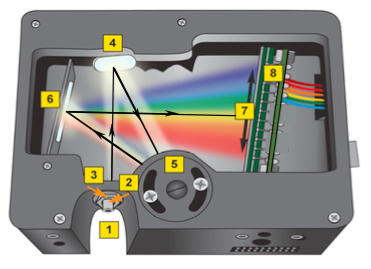
\includegraphics[width=\textwidth]{usb4000.png}
\caption[]{The interior of the USB4000 Spectrograph. Fig. from (Ocean Optics).\footnotemark}
\label{fig: usb4000}
\end{figure}
\footnotetext{\url{http://oceanoptics.com/product/usb4000-custom/}}
}

Light enters the optical bench inside the USB4000 through a light limiting slit (3). If needed the light can be passed through a fiber which connects via the connectors (1-2). A collimating  mirror (4) reflects the light toward the grating. The grating (5) deflects the light on  to a mirror (6) that focus the light on to a lens. The lens (7) focus the light on to the pixels of the CCD detector (8).





















\chapter{Development and Setup of Experiments}
\section{Initial Development}
In order to determine the possibilities and limitations of making observations with a compact spectrograph similar to the USB4000, it was necessary to preform initial testing on the USB4000. 
To examine the spectrograph it was decided to develop different setups to test the stability of the measurements. In an orbit in space the spectrograph will be pointed at different astronomical objects to analyze the light they radiate and thereby analyze the properties of the objects. 

In the laboratory, however, the light source observed by the spectrograph was chosen to be a light source with a very well known spectrum in the wavelength range of the spectrograph. For a well known light source and its spectrum, the laboratory wavelength, which is the wavelength measured in vacuum, of an emission line located in the spectrum is well documented, which enables the spectrograph to be calibrated.  
Upon the development of the setups it was necessary to consider what kind of environment the spectrograph could be subject to if it was launch to space. 

% NOget med MONS satelitte

As mentioned in section \ref{satellite}, the two main common factors for a spacecraft in orbit, are movement due to pointing of the spacecraft and variations of the temperature inside the spacecraft. Furthermore the observations of astronomical objects are often performed over a long duration of time, which means measurements taken over a long period of time must be stable. With these factors taken in to consideration, three experiment setups with different purposes were designed,

\begin{enumerate}
\item Stationary Experiment - Analysis of measurements with the spectrograph being stationary.
\item Simulated Pointing Experiment - Analysis of measurements with the spectrograph with simulation of pointing via vibrations.
\item Temperature Dependence Experiment - Analysis of measurements with the spectrograph at different temperatures.
\end{enumerate}



The development, purpose and improvements of the three experiments and the calibration of the spectrograph will be discussed in the following sections.

\subsection{Calibration of the USB4000 Spectrograph}
The relationship between pixel number and wavelength for the USB4000 is given by a third-order polynomial,\footnote{\url{http://oceanoptics.com/product/usb4000-custom/}}
\begin{equation}
 \lambda _p = I +C_1p + C_2 p^2 + C_3 p^3  ,
 \label{eq: calib}
\end{equation}
where $\lambda_p$ is the wavelength of the pixel \emph{p}, $I$ is the wavelength of pixel 0, and $C_1,C_2,C_3$ are the coefficients of the equation. By using a well known light spectrum with documented spectral emission lines the pixels of the CCD can be calibrated. With the Helium calibration lamp described below, this was done for the USB4000 by taking a measurement of the spectrum from the calibration lamp. The known wavelengths for the spectral emission lines of the lamp, shown in Tbl. \ref{tbl: Helium peaks}, were then fitted to Eq. \ref{eq: calib} with the pixel numbers for the measured lines. The calibration values calculated for the USB4000 are shown in Tbl. \ref{tbl: calib}.

\begin{table}[h]
\centering
    \begin{tabular}{cccc}
    \hline
    $I$ [nm]& $C_1$ [$\frac{nm}{pixel}$]& $C_2$ [$\frac{nm}{pixel^2}$]& $C_3$[$\frac{nm}{pixel^3}$] \\ \hline
    ~
    177.47  & \num{2.2140d-5}    & \num{-6.1407d-6}    & \num{-2.8831d-10}    \\ \hline
    \end{tabular}
    \caption{Calibration values for the USB4000.}
    \label{tbl: calib}
\end{table}

\subsection{Helium Spectrum}
\label{sec: Helium}
To examine the stability of the spectrograph, six spectral emission lines within the Helium spectrum were used. Helium has well known spectral emission lines that are well defined and distributed across the wavelength range of the spectrograph. The use of well defined spectral emission lines ensures that any broadening or shift of the spectral lines are detectable. In Fig. \ref{fig: Helium spectrum} the spectral emission lines in the Helium spectrum in the range 380-900 nm are shown.

\begin{figure}[h!]
\centering
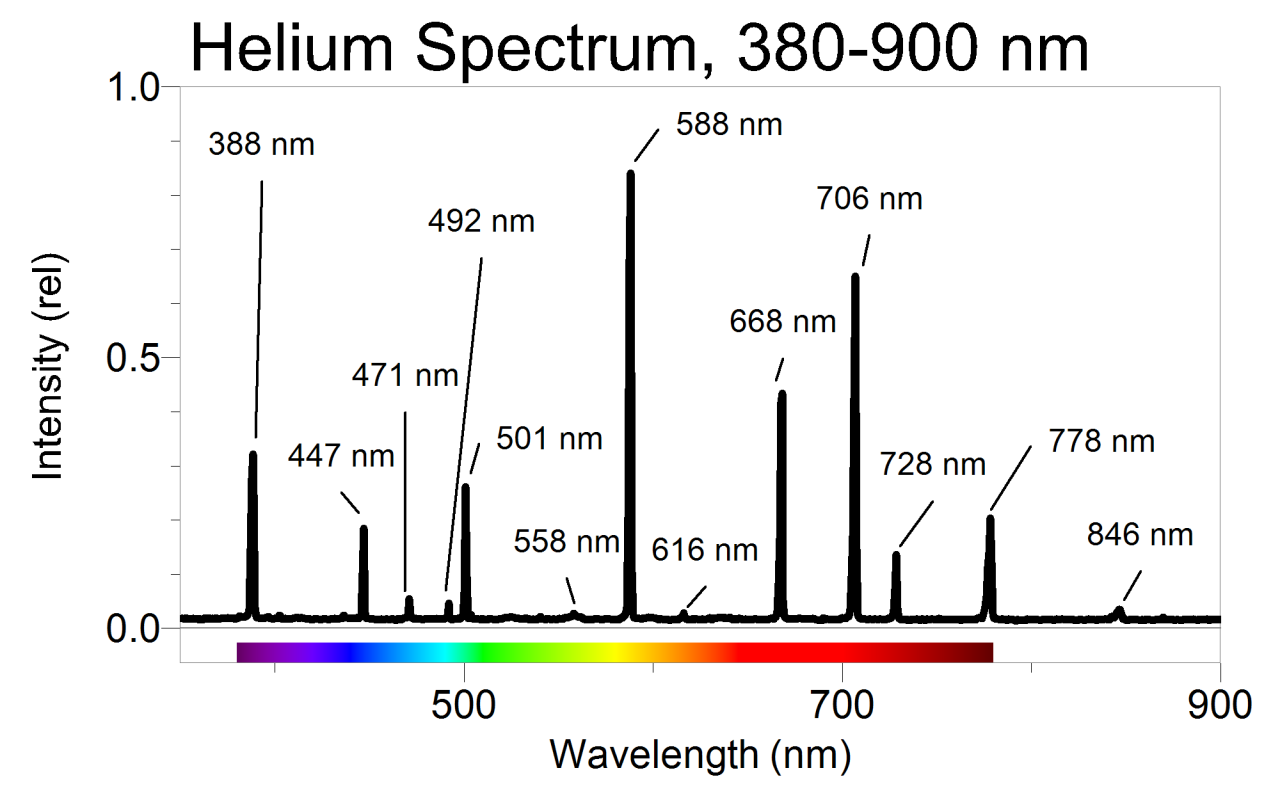
\includegraphics[width = \linewidth]{Helium_spectrum.png}
\caption[]{Spectral lines in the Helium spectrum in the range \SIrange{380}{900}{\nano\m}. Fig. from \citep{helium}.}
\label{fig: Helium spectrum}
\end{figure}



\section{First Experiment- Stationary Measurements}
The purpose of the first setup was to determine the stability of multiple readings over a long period of time from the spectrograph. The parts used for the first initial setup were:

\begin{itemize}
\item HeNe laser
\item  USB4000 Spectrograph with the data acquisition software, \emph{SpectraSuite}\footnote{\url{http://oceanoptics.com/wp-content/uploads/SpectraSuite.pdf}}.
\item Optical bench for mounting the setup
\end{itemize}

The HeNe laser was chosen as the first light source because it had a well documented single peak in its spectrum. The initial setup for the first experiment, is shown in Fig. \ref{fig: First setups}, where a sketch of the setup is illustrated as well as a picture of the actual setup.

\begin{figure}[ht]
\centering
\begin{subfigure}{0.65\linewidth}
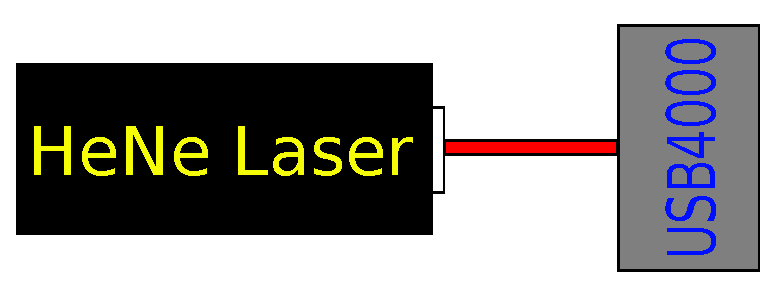
\includegraphics[width=\textwidth]{First_sketch.pdf}
\caption{Sketch of the setup for the first experiment.}
\label{fig: First_sketch}
\end{subfigure}

\begin{subfigure}{0.65\textwidth}
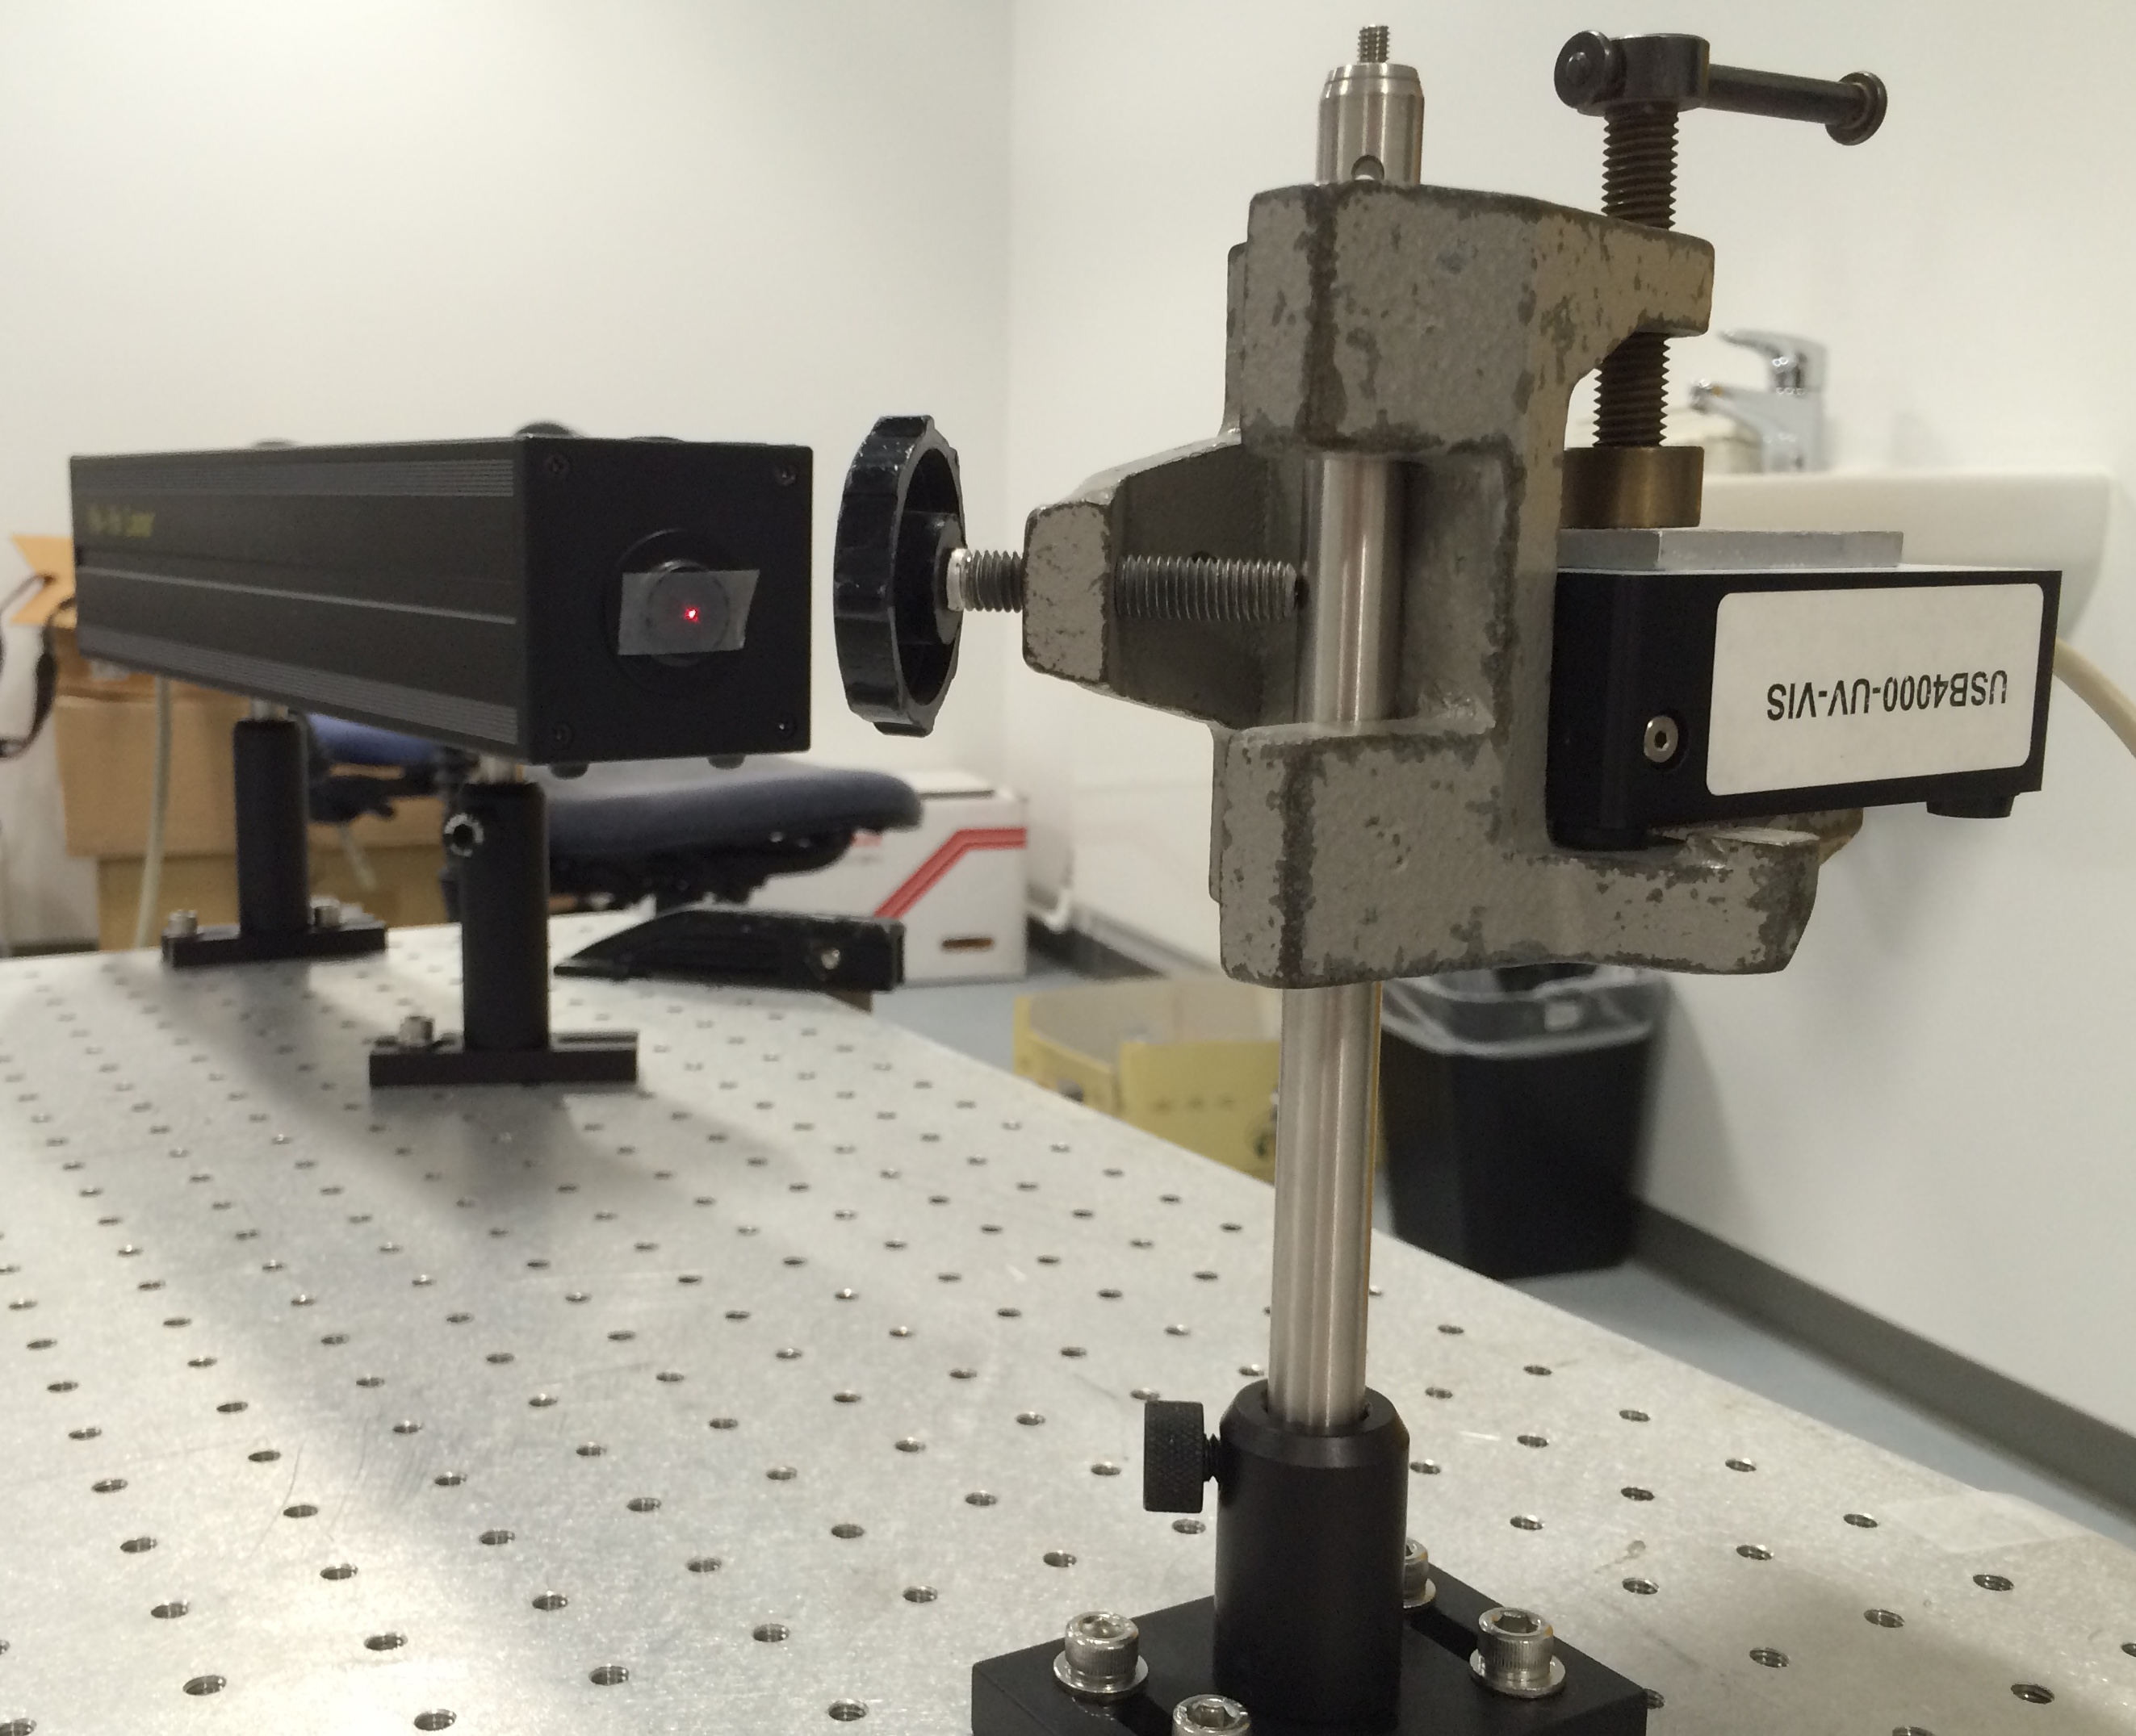
\includegraphics[width=\textwidth]{first_HeNe.JPG}
\caption{Actual setup for the first experiment.}
\label{fig: first_HeNe}
\end{subfigure}
\caption{The setup for the initial run of the stationary measurement with a HeNe laser as the light source. In the top panel a sketch of the top view of the setup is illustrated and in the bottom panel the actual setup is shown from an angle. The tape used as a scrambler is visible over the output lens of the laser.}
\label{fig: First setups}
\end{figure}

The setup for the stationary measurement was very simple as there were no moving parts or control of temperature as was done in later tests. For the execution of the experiment the HeNe laser was aligned so the light beam hit the slit of the spectrograph, which was connected to the data acquisition software, \emph{SpectraSuite}. The laser was fitted with tape across the output lens, this was done because the tape performs like a scrambler which causes the light beam to become more uniform. This was done as an attempt to make the setup less sensitive to alignment of the laser beam on to the spectrograph slit. The parameters for the initial test were,

\begin{itemize}
\item The HeNe Laser was set to an output of \SI{1}{\milli\watt} and the tape was used as a scrambler by placing it over the exit slit of the laser which was pointed onto the entrance slit of the USB4000.
\item In \emph{SpectraSuite} the integration time was set to \SI{10}{\milli\second}, allowing for a high peak to be located at the expected wavelength. Measurements were done every \SI{20}{\second} for a total of \num{1000} measurements.
\item \emph{SpectraSuite} saved the intensity as a function of wavelength to a text file. No filtering of noise from the CCD or smoothing was applied.
\end{itemize}

After the run of the initial setup some problems were found,

\begin{itemize}
\item The results were dependent on the alignment of the laser and the spectrograph. Small vibrations could cause observable changes in the alignment, which caused the laser to saturate the CCD detector, making the measurements useless. 
\item The change in alignment was also able to change the form of the emission line in the measured spectrum to a very flat and wide peak, which was most likely because of internal reflections within the spectrograph.
\item Although the HeNe laser produces a well defined peak, it would be preferable if several peaks located over the range of the spectrograph could be observed, to obtain more data for analysis.
\end{itemize} 

After running the initial setup where the problems mentioned earlier were present, improvements to the setups were introduced. Most of the issues were in someway related to the use of the HeNe laser as the light source. The size of the light spot from the laser was to small compared to the entrance slit of the spectrograph, this meant that the light over the whole entrance slit was not as uniform as desired. In space, movement due to pointing, of the light hitting the slit is expected, but the intensity is not expected to be high enough to saturated the CCD.
\\
\\
For the reasons explained above for the initial setup, the light source used for measurements was changed to a Helium calibration lamp which was used for wavelength calibration as well. In this case several peaks across the measurable range could be selected in the output spectrum to observe for the experiments and the light hitting the entrance slit would be more uniformly spread out due to the lamp no focusing the light on to a small area. Furthermore the mounting to the optical bench was changed in such way that it could be used for the second test as well, which examined the instability of pointing in space via vibrations of the spectrograph. The spectrograph was therefore mounted on top of the shaft of a stepper motor. The stepper motor was mounted with four \SI{90}{\degree} angle pieces onto the optical bench next to the electronics controlling it. The stepper motor was turned off for the stationary test but could be made to move when needed in the second experiment. A sketch and the real setup can be seen in Fig. \ref{fig: setup_vib_final}.

\begin{figure}[h!]
\centering
\begin{subfigure}{0.8\textwidth}
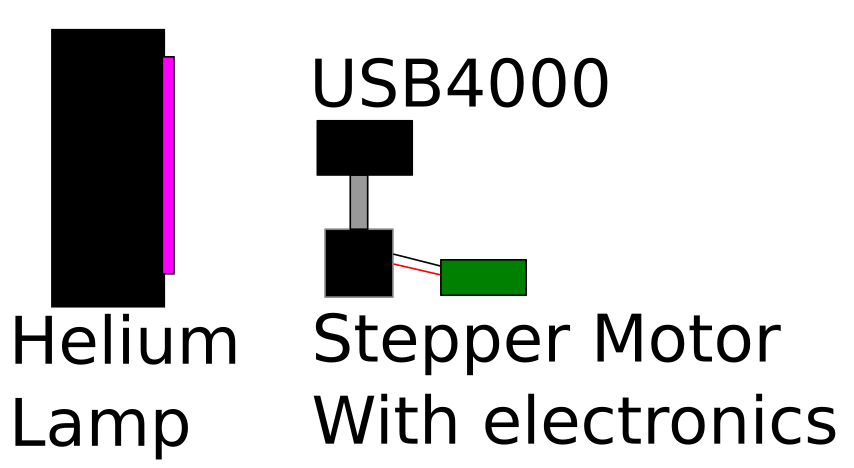
\includegraphics[width=\textwidth]{sketch_vib.png}
\caption{Sketch of setup.}
\label{fig: Vib_sketch}
\end{subfigure}

\begin{subfigure}{0.8\textwidth}
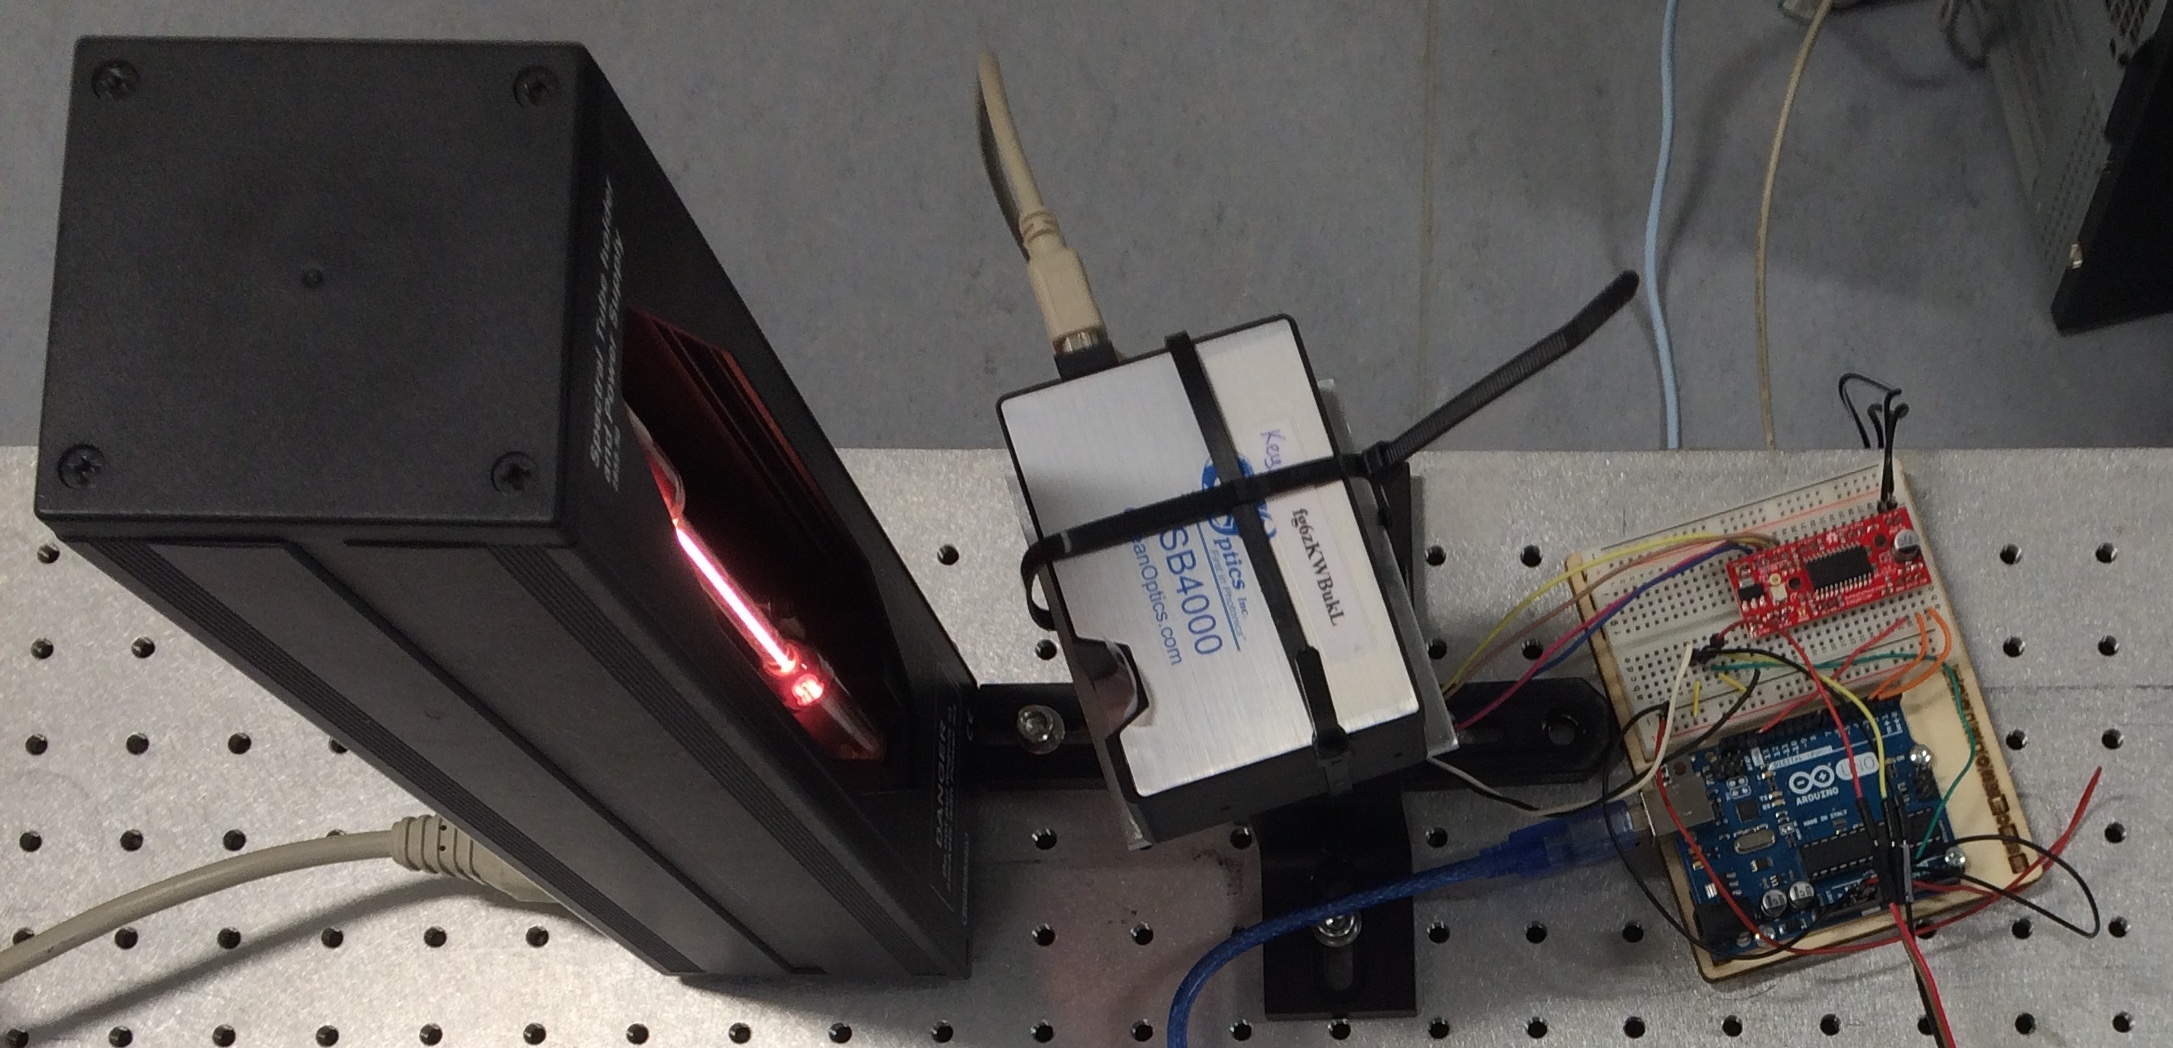
\includegraphics[width=\textwidth]{setup_vib.JPG}
\caption{Actual setup.}
\label{fig: Vib_setup}
\end{subfigure}
\caption{The final setup for both the stationary experiment and simulated pointing experiment. The top panel shows a sketch of the setup seen from the side and the bottom panel shows the actual setup. The electronics were only used to control the stepper motor in the simulated pointing experiment.}
\label{fig: setup_vib_final}
\end{figure}

The change of light source meant that the final parameters of the test were changed,
\begin{itemize}
\item The light source was changed to the Helium calibration lamp. 
\item The tape used as a scrambler was moved to the entrance slit of the spectrograph and the Helium calibration lamp was placed such that the CCD detector in the spectrograph was not saturated.
\item Integration time in \emph{Spectrasuite} was set to \SI{100}{\milli\second}. Measurements were still done every \SI{20}{\second} for a total of \num{1000} measurements, and saved to a text file with the intensity for every wavelength for data processing.
\end{itemize}

\section{Second Experiment - Simulated Pointing}
The purpose of the second experiment was to test the stability of the measurements from the spectrograph, when it was exposed to vibrations, to simulate pointing of the satellite. The setup for the second experiment included the parts used for the final setup in the stationary experiment in addition to,
\begin{itemize}
\item The stepper motor was now used to simulate the pointing of the spacecraft by rotating the spectrograph back and forth over an angle spanning \SI{45}{\degree}. The rotation was done with a frequency of \SI{1.04}{\Hz}, which allowed for enough light exposure at the different angles for the spectrograph to obtain detectable peaks in the output spectrum. 
\item The electronics used to control the stepper motor were the two commercial development boards, \emph{Raspberry Pi} and \emph{Arduino Uno}. These were programmed to moved the stepper motor at the desired frequency.
\item Measurements were taken every \SI{20}{\second} for a total of a \num{1000} measurements. Every measurement was saved to a text file, with the intensity as a function of wavelength.
\end{itemize}

The setup was the same as for the stationary measurement which can be seen in Fig. \ref{fig: setup_vib_final}.

\section{Third Experiment - Temperature Dependence}
The purpose of the third experiment was to determine the temperature dependency of the measurements from the spectrograph. For this experiment it was necessary to build a housing environment were  the temperature could be controlled as precisely as possible. The system would need to be well insulated so the temperature inside could be kept stable for long enough time to allow the temperature of the spectrograph to come in to equilibrium with the set temperature. In orbit the temperature will vary from \SI{-10}{\degreeCelsius} to \SI{40}{\degreeCelsius} on a 90 minute cycle. Because the housing of the spectrograph was not opened the temperature inside can not be measured directly, this is why each temperature is hold for long duration to ensure that the spectrograph is at the set temperature of the housing. Furthermore a window for the light to enter the housing was preferable as this would allow the light source to be placed outside the housing, allowing for a smaller volume in which the temperature needed to be controlled. For the actual heating of the housing and how to control the temperature precisely, different methods were considered,

\begin{itemize}
\item A hot air blower manually set to different temperatures.
\item Thermoelectric cooling by using a Peltier device, which can transfer heat from one side of the device to the other depending on the direction of the current going through it, thereby being able to heat up one of the device sides. 
\item A heater circuit design by ourselves and controlled by a PID temperature controller.
\end{itemize}

For the use of a hot air blower  the housing for the experiment would quickly become complicated to build, to allow for a hot air entrance without a large heat loss, which could cause the temperature to be unstable. A Peltier device is mainly used for cooling purposes by ensuring that the hot side of the device itself is cooled. Thereby allowing the cold side to be cooled even further by transferring its excess heat to the hot side. It would be to time consuming  to develop a setup that worked with precision control of the hot side of the Peltier device. 
\\
\\
Therefore we used a setup using a heater circuit we designed ourselves, that could keep the volume of the housing small and would only need a few wires to be run inside the housing. The heater circuit was controlled by an \emph{Arduino Uno} running PID controller software.
After discussing with the electronics department of Aarhus University Institute for Physics and Astronomy, a simple circuit was designed which satisfied our needs. The circuit schematics can be seen in Fig. \ref{fig: circuit}. The circuit is run of a \SI{12}{\volt} power supply, with the positive terminal connected to a power resistor, functioning as the heating element of the circuit. The high power resistor is capable of having large amounts of power delivered to it, causing it to heat up as current flows through it and as the voltage drops across it. The resistor was connected to ground through a transistor controlled by the \emph{Arduino Uno}. The transistor works as a switch, which connects the collector and emitter legs of the transistor when a voltage is applied to the base leg. The resistor was connected to the collector leg and the emitter leg was connected to ground, while the base leg was connected to the \emph{Arduino Uno} with the PID software. The PID software  controlled when and for how long the collector and emitter legs were connected based on the temperature readings from a temperature sensor connected to the \emph{Arduino Uno} from inside the test housing. With the wanted temperature inside the housing being adjustable from the PID software, the experiment could be run without the need to physical interrupt the setup. 
\\
\\
After deciding on a wanted design, an initial test setup was build to ensure the heating circuit and PID controller were working as planned. The setup was constructed with the following parts:
\begin{itemize}
\item The housing was made from a small cardboard box, as high insulation was not needed for testing if the heater circuit and PID controller worked as expected. This setup is shown in Fig. \ref{fig: cardboard}.
\item A 12 V power supply, BD649 Transistor, SH650 Resistor and TMP35 Temperature sensor.\footnote{Component Data sheets : \url{http://www.alldatasheet.com}}
\end{itemize}

\begin{figure}[h]
\centering
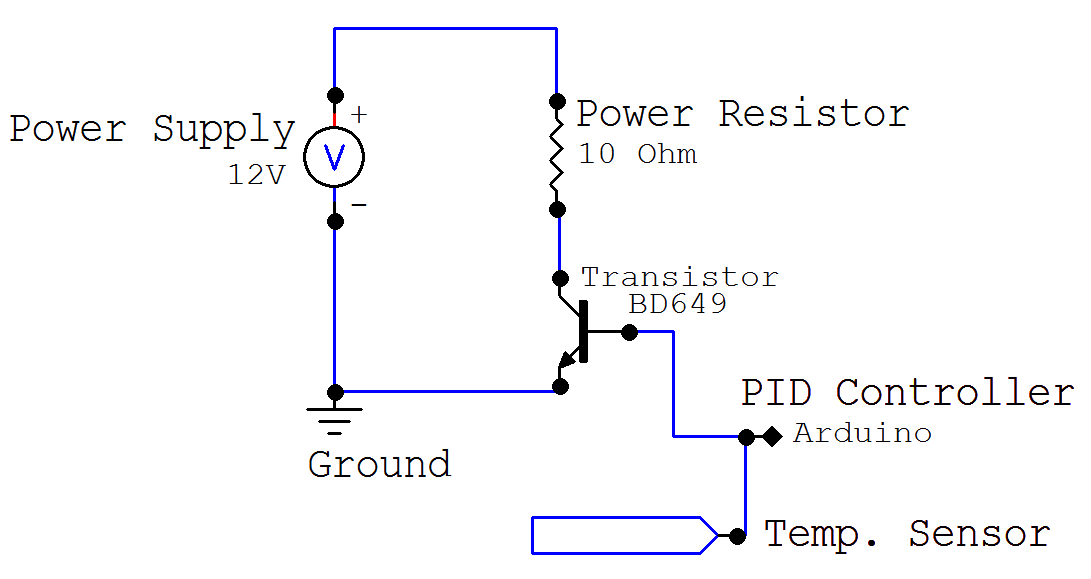
\includegraphics[width =\linewidth]{kredslob.png}
\caption{Schematic view of the heater circuit used to control the temperature in the housing for the temperature dependence experiment.}
\label{fig: circuit}
\end{figure}

The spectrograph was placed in the housing with a window for the light to enter. Tape was used to insulate the window and works as a scrambler like in the previous experiments. The power resistor was mounted on a heatsink in contact with the spectrograph, the temperature sensor was mounted on the spectrograph as well. The power resistor and temperature sensor were mounted directly onto the spectrograph because it was expected to provide the fastest heating and most stable temperature readings. A small fan was put in the housing to circulate the air to get a uniform temperature inside the housing. The cables were then run outside the housing to the remaining circuit. The setup inside and outside the housing is shown in Fig. \ref{fig: cardboard}.

\begin{figure}[h!]
\centering
\begin{subfigure}{.5\textwidth}
\centering
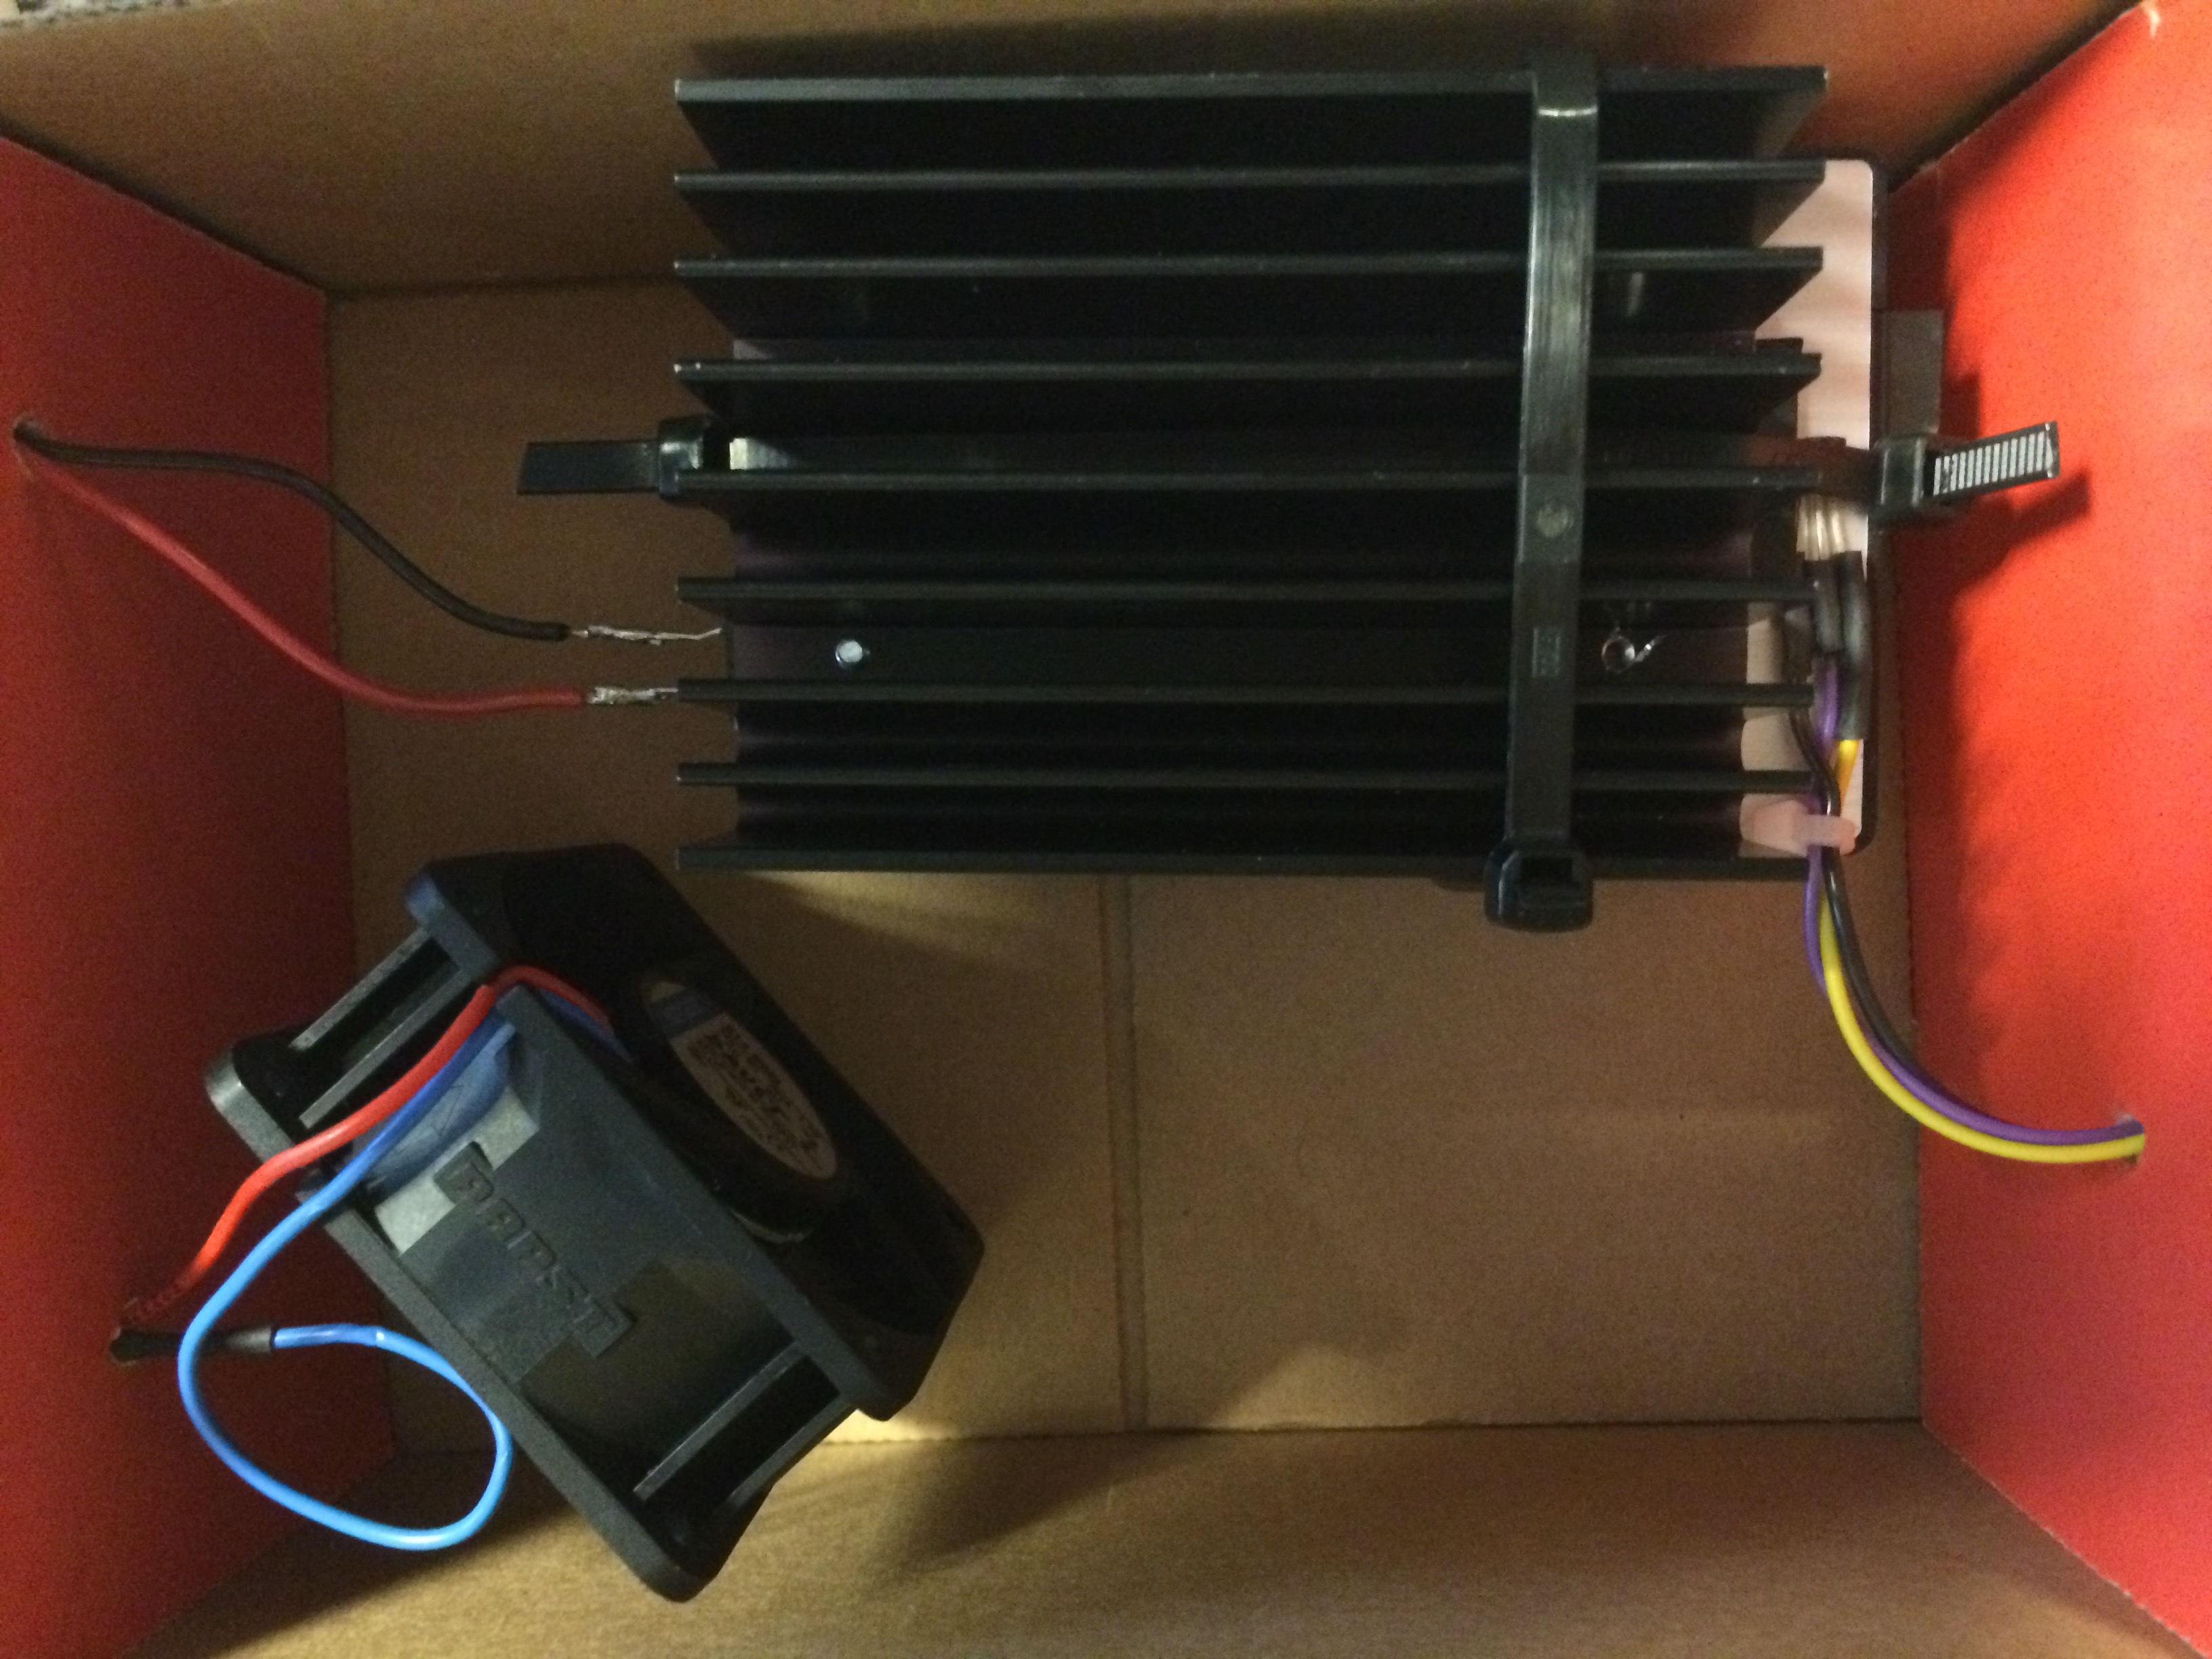
\includegraphics[width=.95\linewidth]{cb_circuit.JPG}
\caption{Inside of housing.}
\label{fig: cd_circuit}
\end{subfigure}%
\begin{subfigure}{.5\textwidth}
\centering
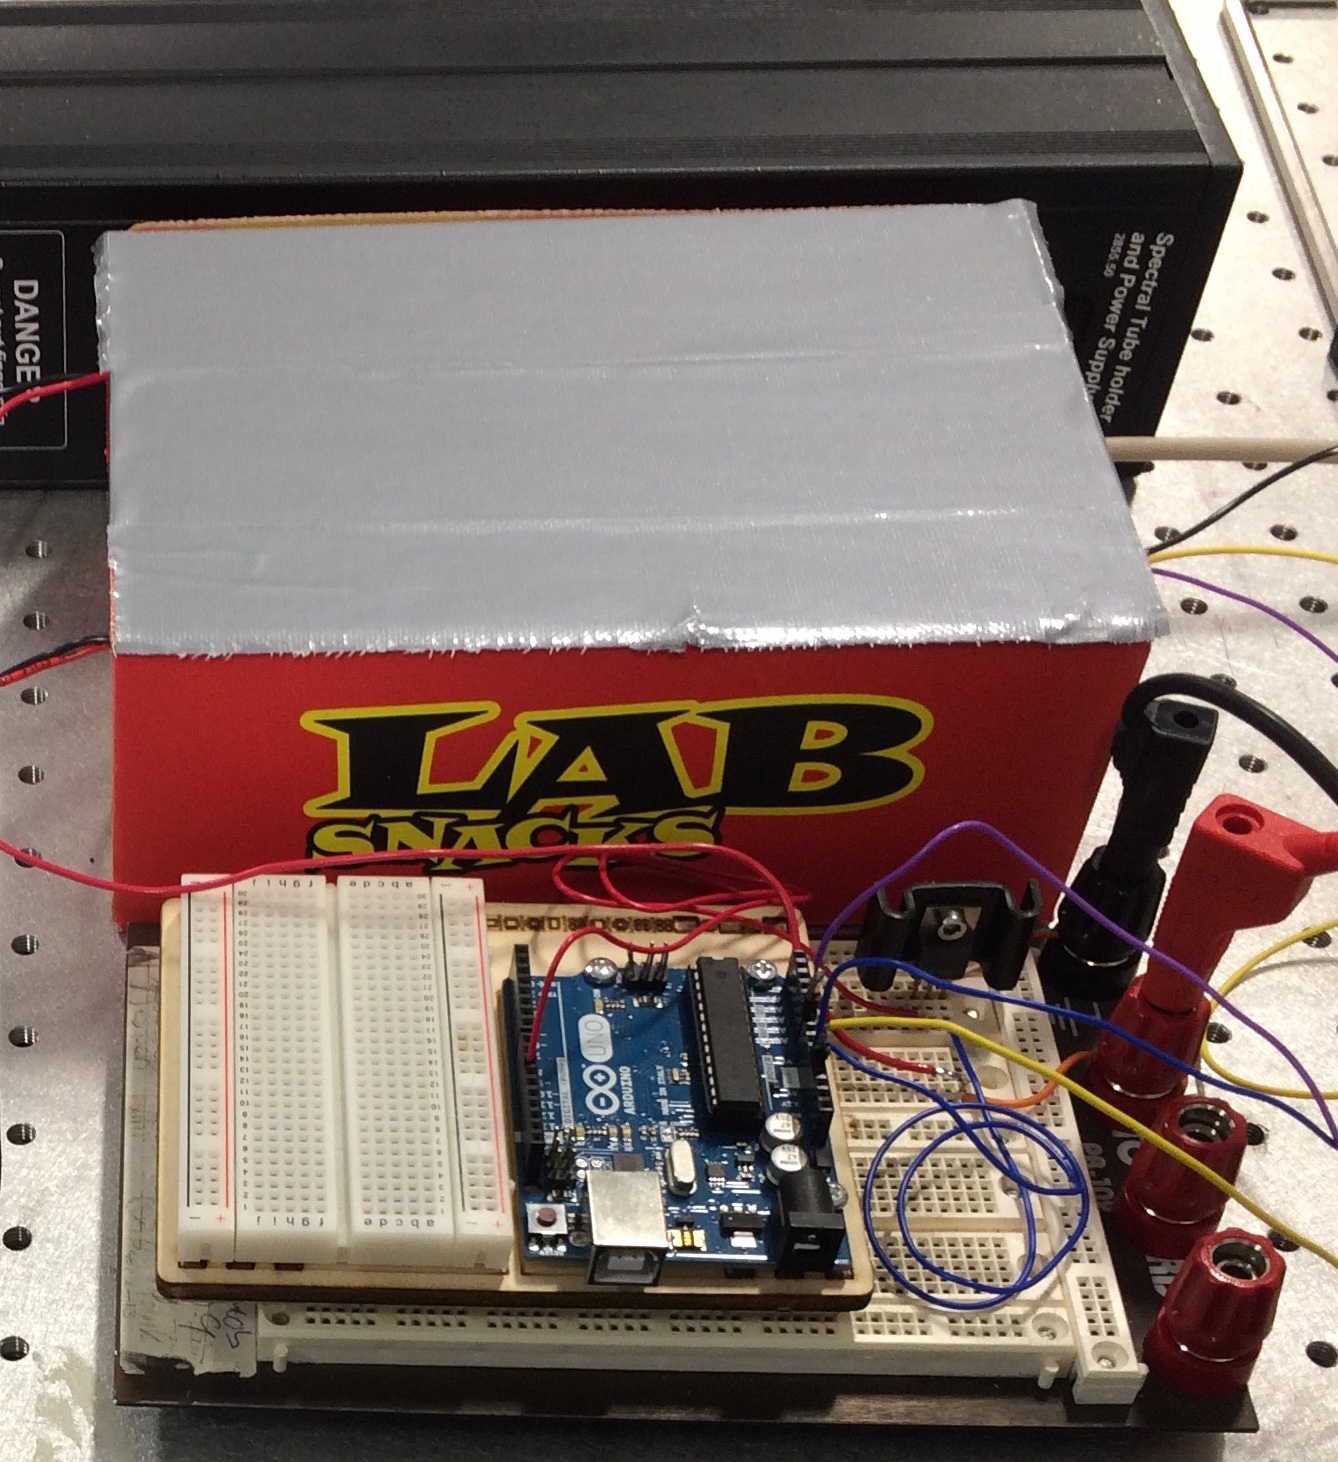
\includegraphics[width=.9\linewidth]{outer_circuit.JPG}
\caption{Outside view of the circuit test.}
\label{fig: outer_circuit}
\end{subfigure}
\caption{The inside and outside view of the setup to test the heater circuit and PID controller. The left panel shows the resistor with heatsink  and the temperature sensor mounted on top of the spectrograph as well as the fan for circulating the air. In the right panel the outside of the setup is shown, including the Helium lamp in the background, the part of the heater circuit located outside the housing.}
\label{fig: cardboard}
\end{figure}

After conducting the initial test of the heater circuit and PID controller some adjustments were made for the final setup to improve stability of the temperature in the housing,
\begin{itemize}
\item The housing was changed to a Styrofoam box for better insulation allowing the set temperature to be reached faster.
\item The resistor and temperature sensor were moved so they were not in contact with the spectrograph, but instead the heating and temperature measurements were done on the circulating air. This was done because it allowed for a more stable temperature within the housing.
 
\end{itemize}

The final setup for the third experiment with the mentioned improvements is shown in Fig. \ref{fig: temp setup final}.
\\
\\
\begin{figure}[h]
\centering
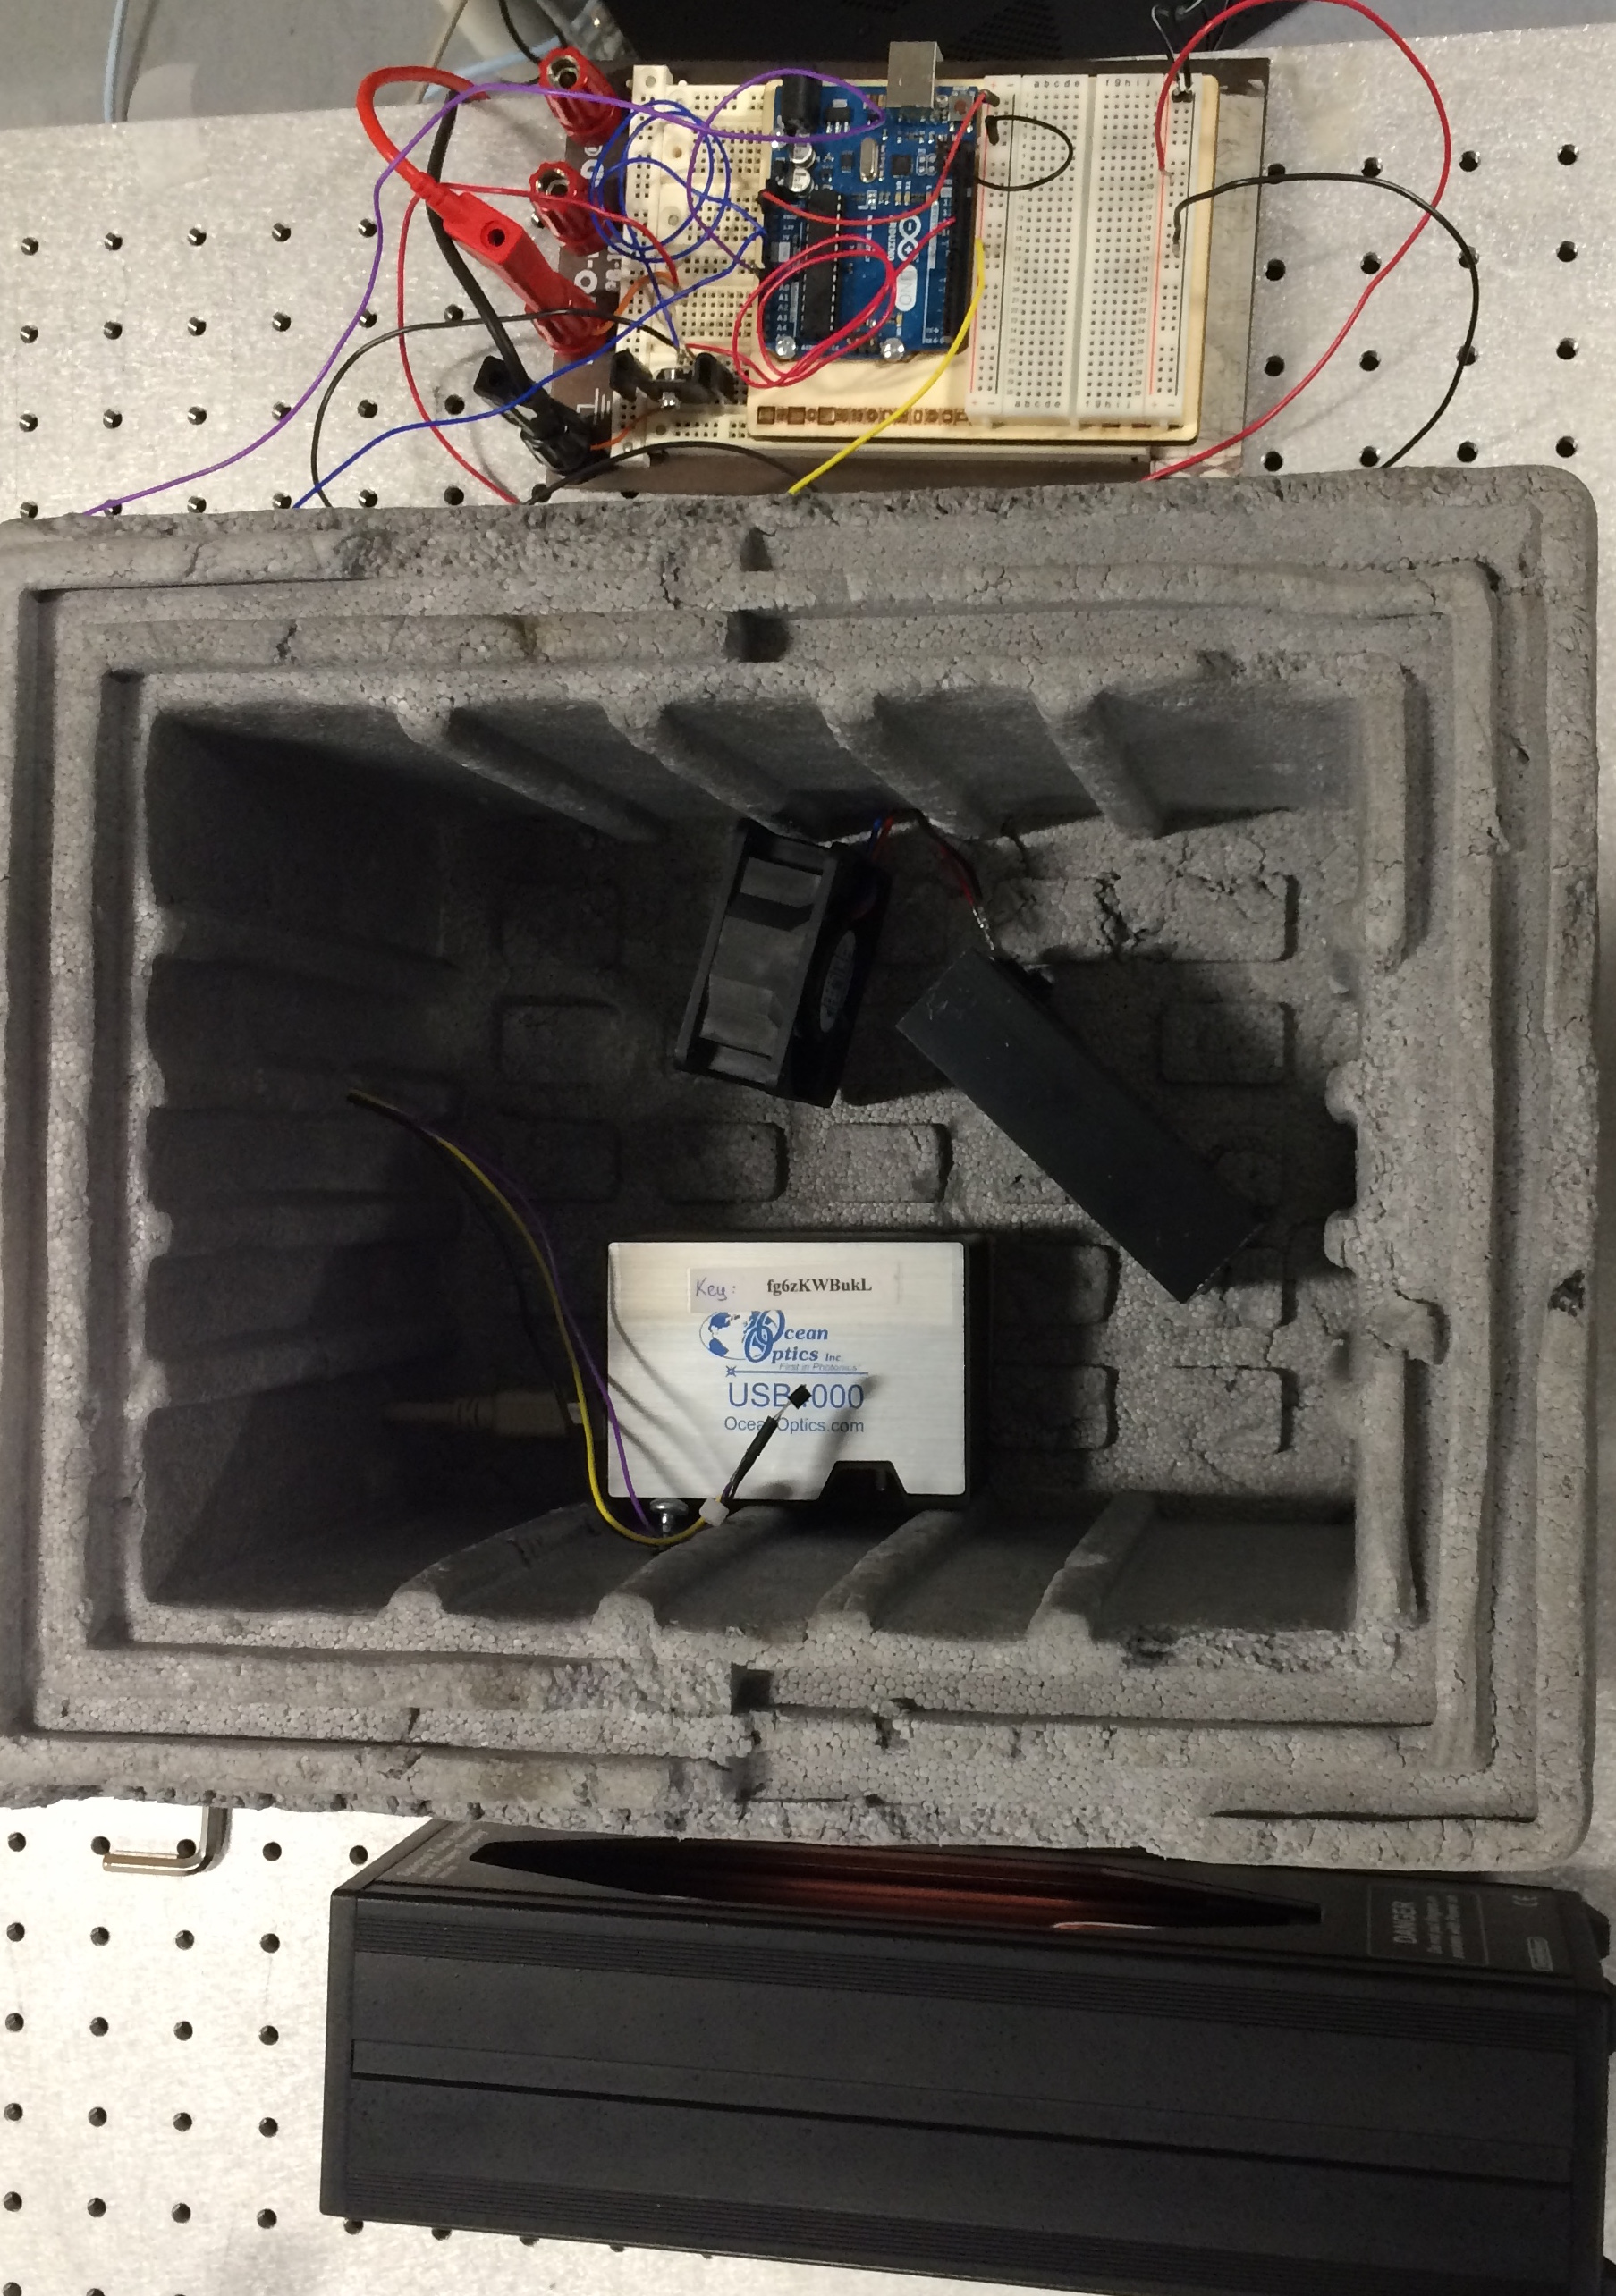
\includegraphics[width=.45\linewidth]{flamingo_circuit.JPG}
\caption{The final setup used for the third experiment. The spectrograph was placed with the entrance slit aligned with the window made in the side of the housing. The resistor with heatsink was placed in front of the fan so the circulating air was heated and the temperature sensor was placed so it measured the air temperature. The housing was closed of with a lid when the experiment was run.}
\label{fig: temp setup final}
\end{figure}

With the final setup decided upon the third experiment was run with the parameters,
\begin{itemize}
\item Measurements were made with the temperature varying from \SI{19.5}{\degreeCelsius} to \SI{49.3}{\degreeCelsius} in eleven steps. Because the spectrograph was heated by the circulating air, the temperature was hold steady for each step for two hours to allow for uniform temperature in the spectrograph.
\item Integration time in \emph{SpectraSuite} was set to \SI{100}{\milli\second} and measurements were taken every \SI{1}{\second} for a total of \num{60} measurements for every temperature step. The intensity of every wavelength was saved to a text file for data processing. 
\end{itemize}






\chapter{Results}

\section{General method of data processing}

The Helium spectrum from each measurement was saved to a text file, which included wavelengths with corresponding photon count. As an example of the Helium spectrum the unfiltered data with background noise, from a stationary measurement are shown in Fig. \ref{fig: demo data with noise}. 

\begin{figure}[h!]
\centering
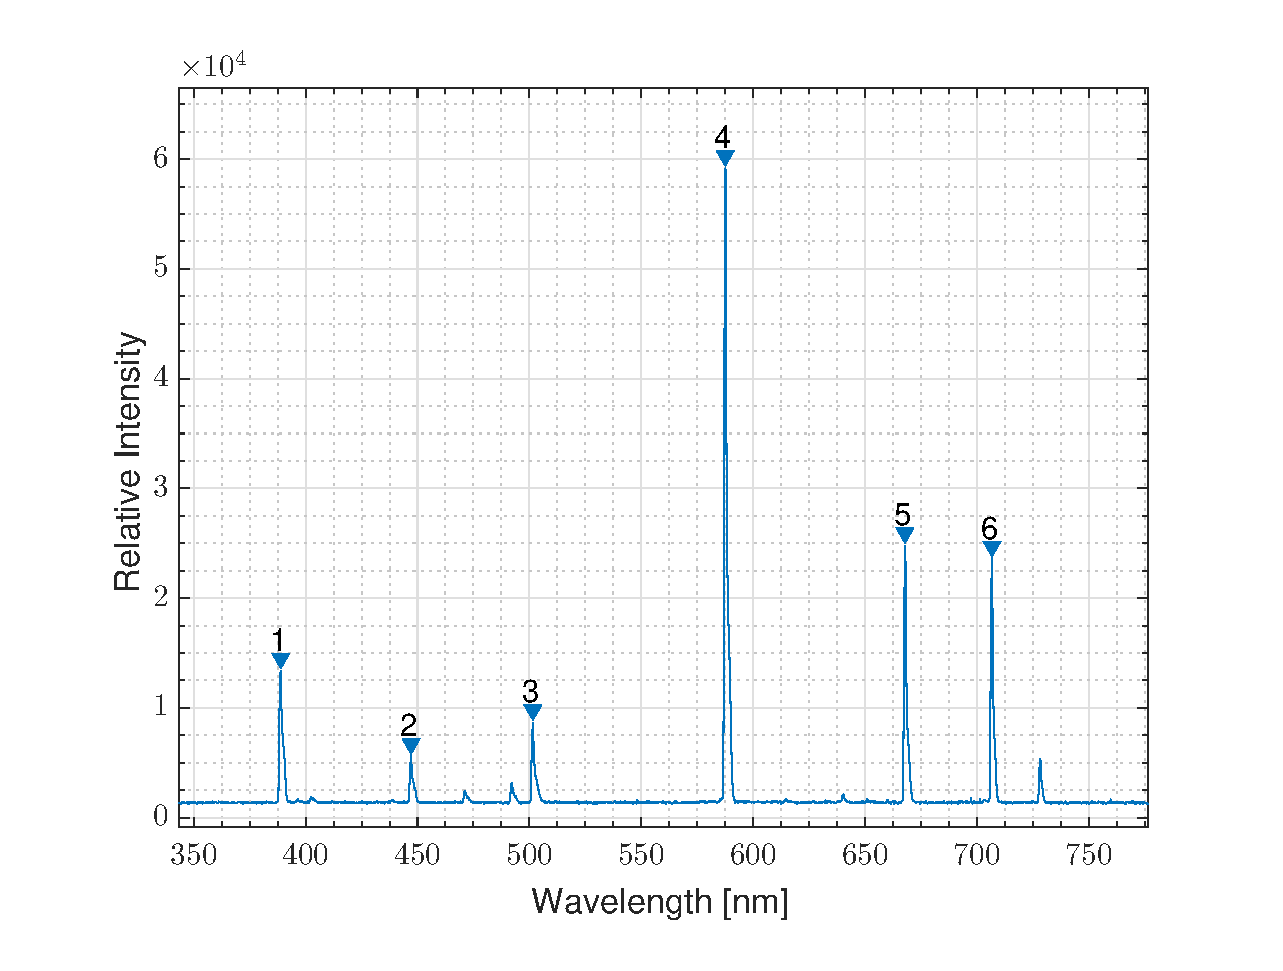
\includegraphics[width=\linewidth]{figures/spectrum_with_noise_numbered.eps}
\caption{Example of the Helium spectrum from a measurement with the spectrograph, here illustrated by a spectrum from a stationary measurement. The six peaks that were used to determine the stability of the centroid wavelength value are marked and numbered one to six starting from the peak with the shortest wavelength.}
\label{fig: demo data with noise}
\end{figure}




The six emission lines used to determine the stability of the spectrograph for all three experiments, are marked and numbered from one to six in Fig. \ref{fig: demo data with noise} with the numbering starting from the peak with the shortest wavelength. The corresponding laboratory wavelength to peak number are shown in Tbl. \ref{tbl: Helium peaks}.
\begin{table}
\centering
    \begin{tabular}{cc}
    \hline
    Peak number & Wavelength [nm] \\ \hline
    1           & 388.86           \\
    2           & 447.14         \\
    3           & 501.58           \\
    4           & 587.56         \\
    5           & 667.82           \\
    6           & 706.52           \\ \hline
    \end{tabular}
    \caption{Wavelengths for the six spectral emission lines that were used in the experiments of this thesis \citep{helium-wavelength}.} 
    \label{tbl: Helium peaks}
\end{table}

The data from all measurements within each experiment firstly had the background noise from the CCD sensor removed. The background noise needed to be removed before is was possible to fit any functions to the data. This is done by using the intensity for wavelengths below 350 nm, where no spectral line are present from Helium, here only the noise on the CCD sensor is present, the average of the measured intensity for all wavelengths below \SI{350}{nm} was subtracted from the relative intensity for all data as the noise was uniform for the total wavelength range.
Then for every measurement the six marked peaks in Fig. \ref{fig: demo data with noise} will be found within each spectrum, and a Gaussian function will be fitted to each peak to determine the centroid wavelength of all the peaks. These wavelengths will be compared within all three experiments. Peak number 4, located around \SI{587}{nm}, was used in all three experiments to illustrate the data processing.

The general form of a Gaussian function is:
\begin{equation}
f(x) = A exp\left(-\frac{(x-b)^2}{2  \sigma^2}\right),
\label{eq: Single Gaussian}
\end{equation}
where, $A$ is the amplitude, $b$ is the centroid value of the peak and $\sigma$ is the standard deviation, which determines the width of the Gaussian profile.
\\
\\
The typical form of a peak with a fitted Gaussian function is shown in Fig. \ref{fig: double gauss}. It can be seen that the peak has a "shoulder" on the right which can be easily fit by two Gaussian. This is illustrated in Fig. \ref{fig: two single gauss}. %It is so because the peak is actually made up of two Gaussian functions that overlap, this is shown in fig. \ref{fig: two single gauss}, where the two single Gaussian functions that make up the combined Gaussian function, are illustrated separately. 
From section \ref{sec: Helium} it is known that the spectral lines of Helium are well defined. The distance between the two peaks was constant for all the lines in every measurements, which indicates that the "shoulder" of the spectral line is most like caused by internal reflections within the spectrograph. To determine the specific cause of this broadening, it would be necessary to take the spectrograph apart and do further testing. This is beyond the scope of this bachelor's thesis but the broadening will be filtered out in the data processing. 
\\
\\
To accurately identify the centroid of the peak, to be measured, it is necessary to fit to a combination of two Gaussian functions of the form:
\begin{equation}
f(x) = A_1 exp\left(-\frac{(x-b_1)^2}{2 \sigma_1^2}\right) + A_2 exp\left(-\frac{(x-b_2)^2}{2\sigma_2^2}\right),
\label{eq: Double Gaussian}
\end{equation}
and when a fit in the form of Eq. \ref{eq: Double Gaussian} has been found, we are able to get the information about the two separate Gaussian functions and thereby get the centroid information about the narrow and tall peak in which we are interested. 
\\
\\
One way to determine the uncertainty for every found wavelength is to use the \emph{Full Width at Half Maximum} (FWHM), which is the the width of the peak at half the maximum amplitude. FWHM is determined by the standard deviation, $\sigma$. The relationship between the two is given by:
\begin{equation}
FWHM = 2\sqrt{2ln2}\sigma,
\label{eq: FWHM}
\end{equation}
where $\sigma$ is obtained from the Gaussian function fitted to every peak.

\begin{figure}[h!]
    \centering
        \begin{subfigure}{0.5\textwidth}
        \centering
        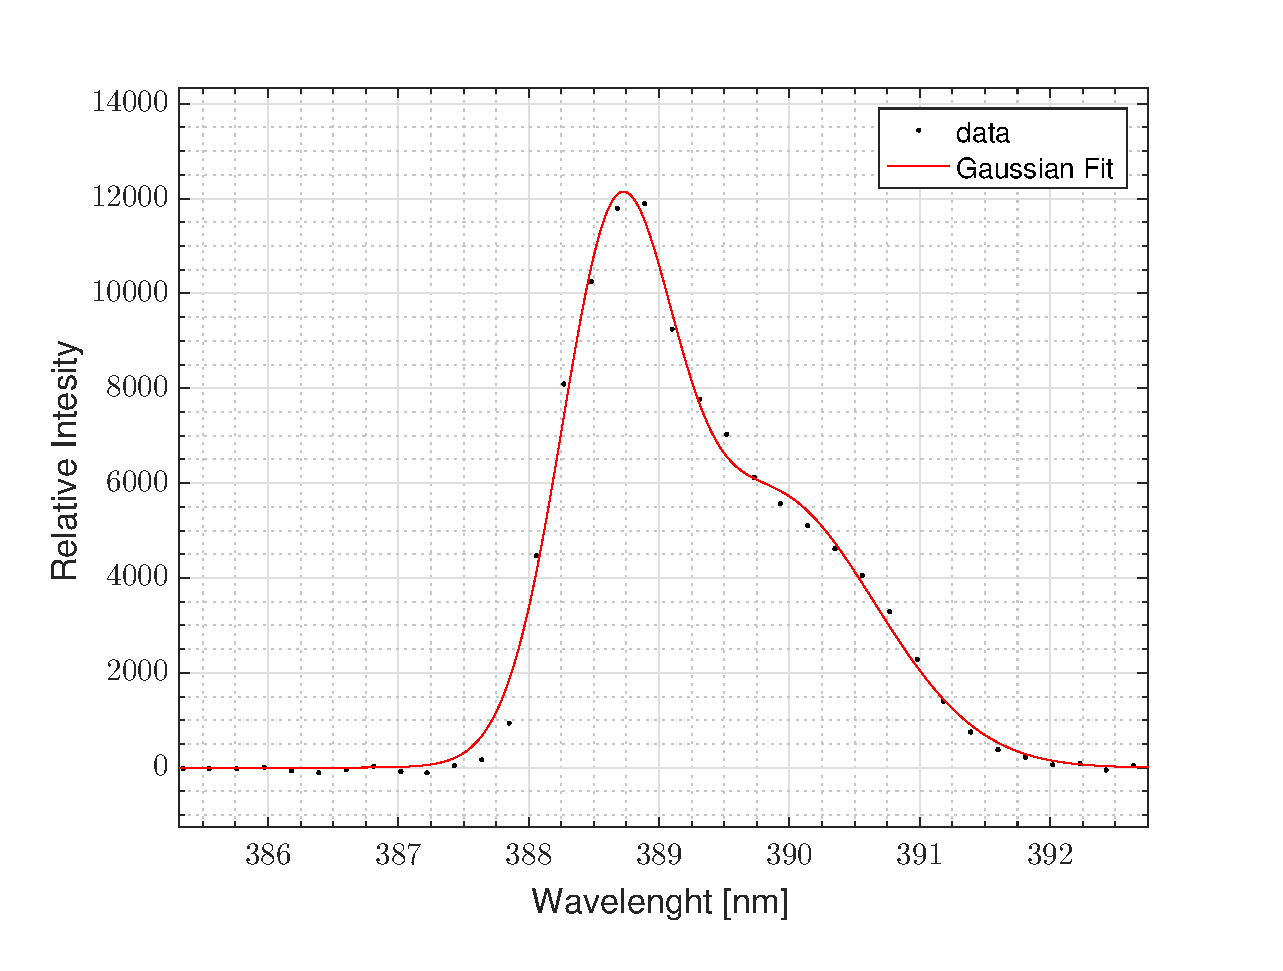
\includegraphics[width=\linewidth]{figures/typisk_dobbelt_gauss.eps}
        \caption{Typical peak form, with double Gaussian fitted.}
        \label{fig: double gauss}
    \end{subfigure}%
    ~
    \begin{subfigure}{0.5\textwidth}
        \centering
        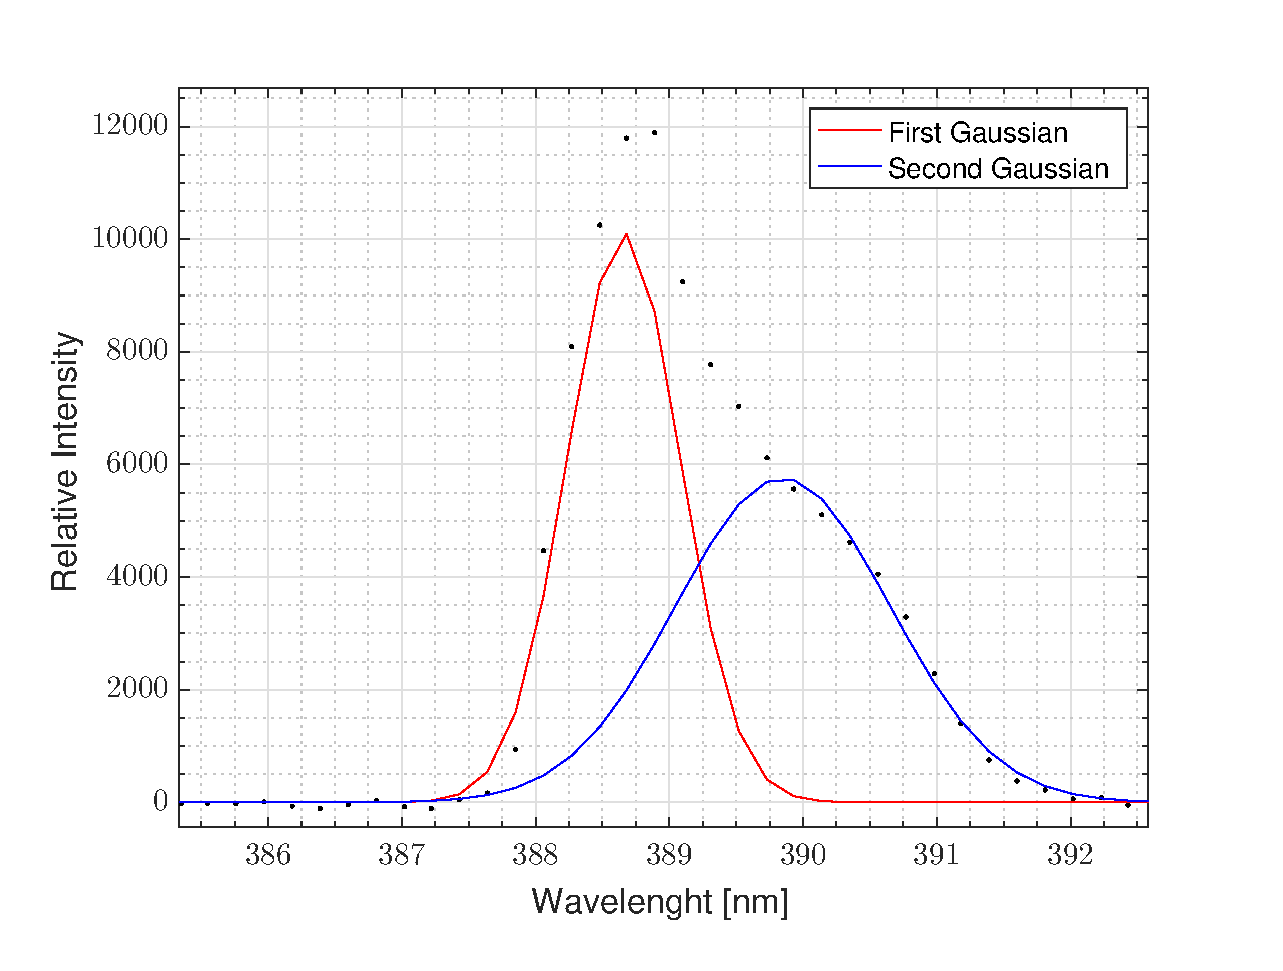
\includegraphics[width=\linewidth]{figures/to_enkelt_gauss.eps}
        \caption{The two single Gaussian functions that make up the fit in Fig. \ref{fig: double gauss}.}
        \label{fig: two single gauss}
    \end{subfigure}%
    \caption{Overview of the general observed Gaussian peak form. The left panel shows the form of the two combined Gaussian functions that are fitted to the experimental data and the right panel shows how the combined Gaussian can be split up into two single Gaussian functions. }
    \label{fig: Demo gauss peaks}
\end{figure}


Another way of determining the uncertainty is possible if an average of multiple measurements is done. Averaging multiple measurements is a practice often used when making observations from space. In space, observations are more prone to noise from radiation hitting the CCD sensor than on Earth, due to higher radiation in space. By stacking measurements, a single measurement with an increased value due to cosmic radiation hitting the CCD detector is less prominent and thereby reduces the uncertainty of the measured wavelength.
From $n$ measurements, the average, $\bar{x}$, and the standard deviation can be calculated from,

\begin{align}
\bar{x} = \frac{1}{n} \sum^{n}_{i=1}x_i,
\label{eq: avg}
\end{align}
\begin{align}
\sigma = \sqrt{\frac{1}{n-1} \sum_{i=1}^{n} (	x_i-\bar{x} )^2}.
\label{eq: std}
\end{align}
From the standard deviation the uncertainty, $S_{\bar{x} }$, of the average can be calculated,
\begin{align}
S_{\bar{x} } = \frac{\sigma}{\sqrt{n}} 
\label{eq: Sx}
\end{align}

\section{First Experiment - Stationary Measurements}

For the first experiment, code was written in \texttt{Matlab} to analyze all the measurements. In the data from every measurement the six peaks mentioned in Tbl. \ref{tbl: Helium peaks} were found. Each of the six peaks were then fitted to a function of the form seen in Eq. \ref{eq: Double Gaussian}. The parameters obtained from the fit were analyzed in order to identify which belonged to the narrow and taller peak. The parameters were analyzed by comparison of their amplitudes, and making sure that any fits with a negative amplitude were redone with limitations on the fitting parameters. Also the centroid parameters, which should have a constant distance to each other, were compared to make sure the fittings were done properly. With these parameters it was possible to fit a function of the form seen in Eq. \ref{eq: Single Gaussian}, to the data, where the measured noise from the earlier discussed "shoulder" Gaussian, was filtered out. The fit to a single Gaussian allowed for a more narrow width of the peak, which led to a smaller FWHM value and thereby a smaller uncertainty on the found wavelengths.
\\
\\
After the six emission peaks had been found in all measurements, outliers that had not been fitted properly by the code were removed from the data. Bad fittings were visible in the FWHM values. All the lines that had been fitted correctly had FWHM values around \SI{1}{nm}, while the badly fitted peaks had FWHM values above \SI{2}{nm}. The data filtered out by high FWHM values were less than \num{10}\% of the total measurements.
\\
\\
The measured wavelengths for each peak were then plotted against the time from the start of the experiment. For peak number 4, all the measured wavelengths are shown in Fig. \ref{fig: exp1 1000 maalinger} and the uncertainties in form of the FWHM for the measured wavelengths are shown in Fig. \ref{fig: exp1 1000 fwhm}. These are of the order of \SI{1}{nm}, when Eq. \ref{eq: FWHM} was used.


\begin{figure}[h!]
\centering
\begin{subfigure}{.9\textwidth}
\centering
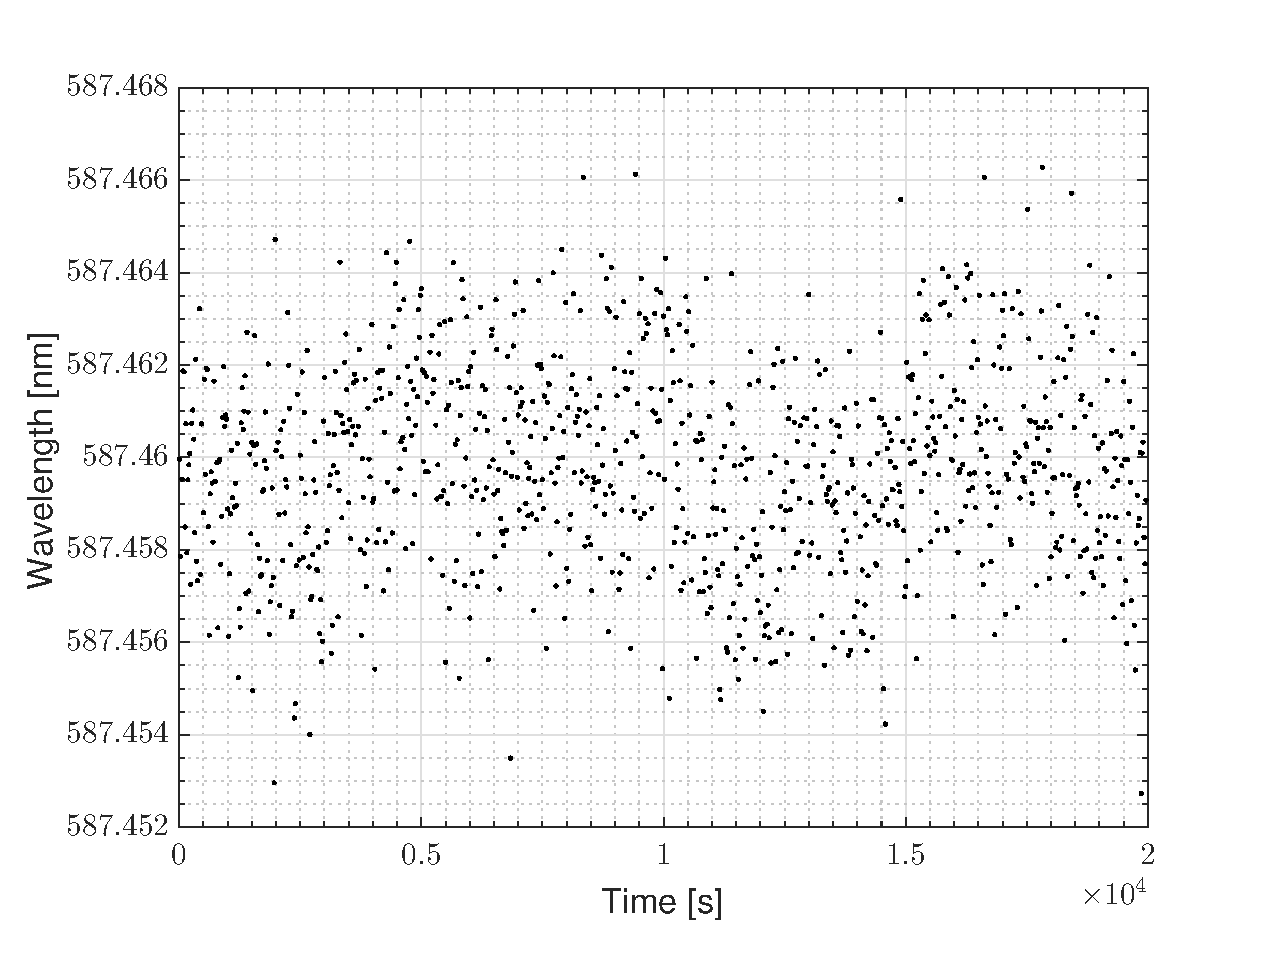
\includegraphics[width = \linewidth]{stat_587_1000_maalinger.eps}
\caption{Measured wavelengths over time.}
\label{fig: exp1 1000 maalinger}
\end{subfigure}
\begin{subfigure}{.9\textwidth}
\centering
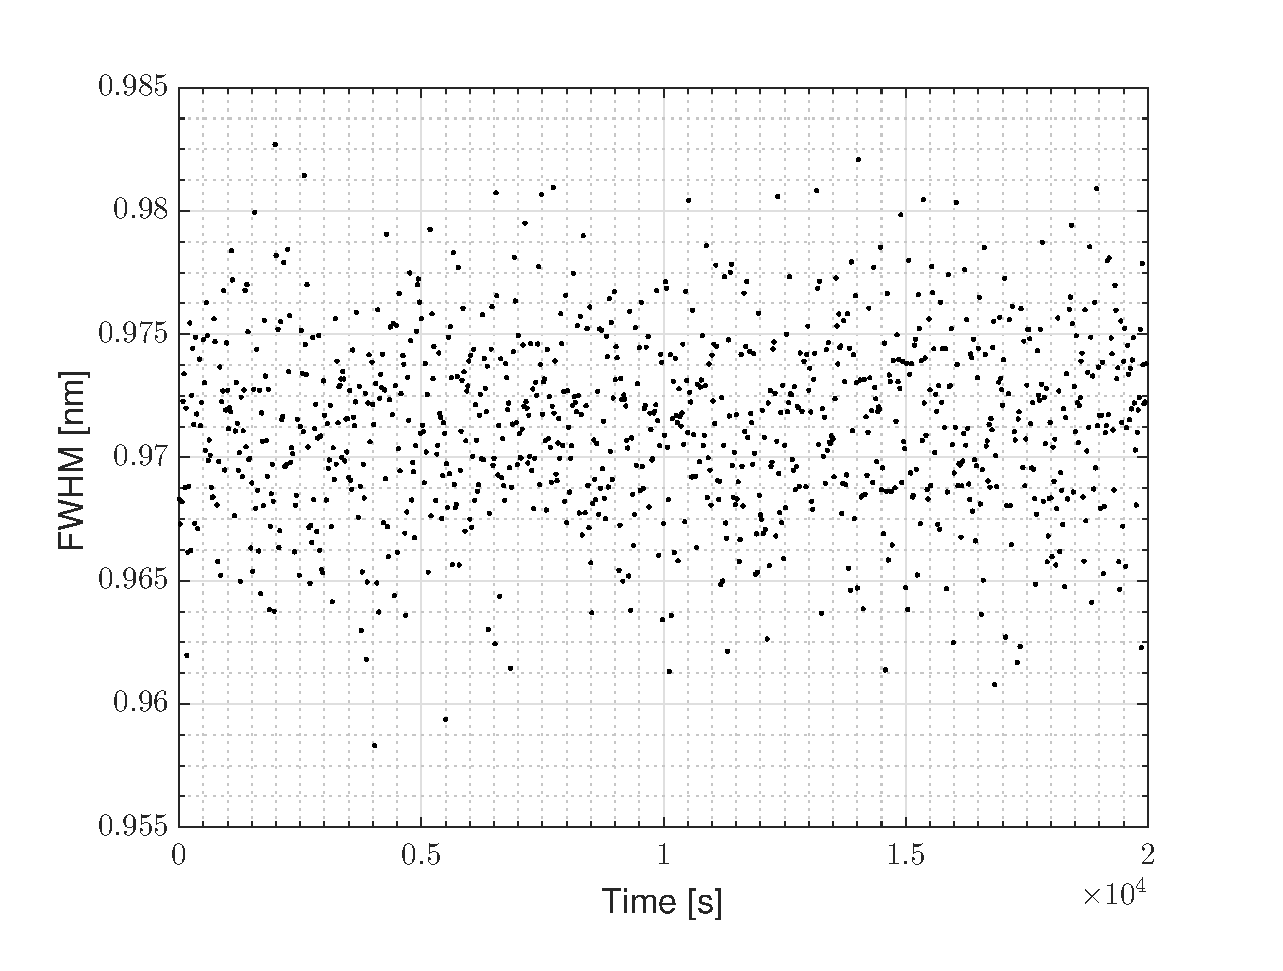
\includegraphics[width = \linewidth]{stat_587_fwhm.eps}
\caption{FWHM for wavelengths over time.}
\label{fig: exp1 1000 fwhm}
\end{subfigure}
\caption{In the top panel the measured wavelengths, for peak 4, from thousand measurements are shown over time. In the bottom panel the FWHM values for the wavelengths, for peak 4, are shown. }
\label{fig: Exp1 1000 samlet}
\end{figure}

The measurements were then binned to contain twenty measurements each and were analyzed using standard deviation described in Eq. \ref{eq: avg}, \ref{eq: std} and \ref{eq: Sx}. The average of each bin was calculated and the uncertainty was calculated from Eq. \ref{eq: Sx}. The measured wavelengths over time are shown in Fig. \ref{fig: exp1 bins} along with the calculated uncertainties.

The last processing of the data from the first experiment was done by taking the average of all the measured wavelengths for each peak. Then the uncertainty of the average for each peak was found. The average peak wavelengths are shown in Tbl. \ref{tbl: exp1 values} where they can be compared to the laboratory wavelengths of the peaks. The uncertainty for each emission line is shown in Fig. \ref{fig: exp1 usikkerhed peaks}.

\begin{figure}[!ht]
\centering
\begin{subfigure}{0.9\textwidth}
\centering
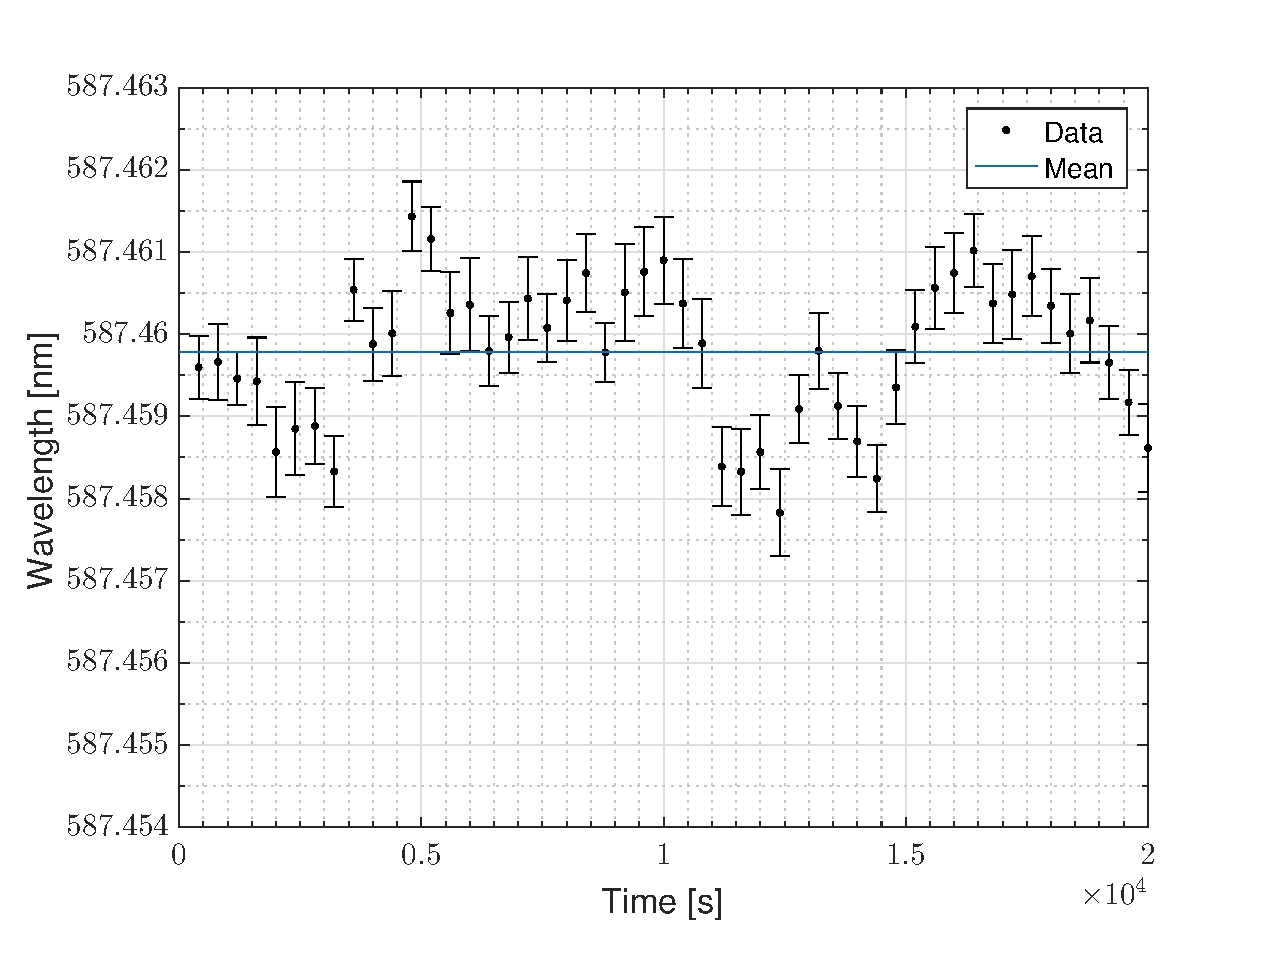
\includegraphics[width = \linewidth]{stat_587_bins_med_usikkerhed.eps}
\caption{Wavelengths measured when the measurements were binned.}
\label{fig: exp1 bins}
\end{subfigure}
~
\begin{subfigure}{0.9\textwidth}
\centering
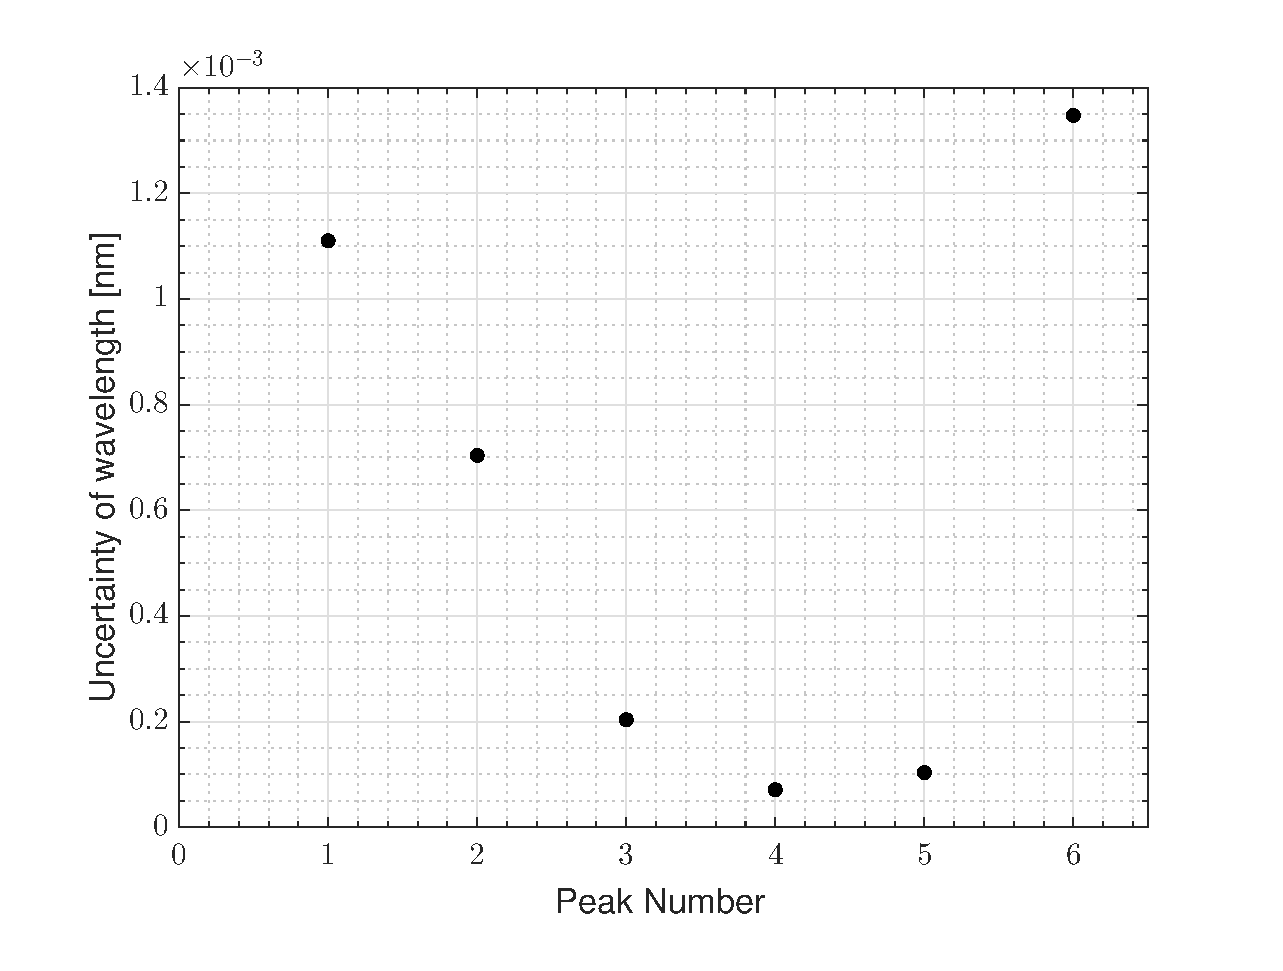
\includegraphics[width = \linewidth]{stat_usikkerhed_alle.eps}
\caption{The uncertainty of the average wavelength for every peak.}
\label{fig: exp1 usikkerhed peaks}
\end{subfigure}
\caption{In the top panel the average wavelengths for bins containing twenty measurements are shown over time. The uncertainty of each wavelength is illustrated with errorbars. In the bottom panel the uncertainty of the total average wavelength measured for each peak is shown.}
\label{fig: exp1 samlet bins}
\end{figure}

\begin{table}
%\centering
\centerline{
    \begin{tabular}{ccccc}
    \hline
    Peak number & Average Wavelength [nm] & Laboratory Wavelength & $\Delta\lambda$ [nm]& $S_{\bar{x}}$ [$10^{-3}$ nm] \\ \hline
    1           & 389.02                  & 388.86      &    0.16      & 1.1                     \\
    2           & 447.22                  & 447.14       &    0.08     & 0.7                     \\
    3           & 501.56                  & 501.58        &    0.02    & 0.2                     \\
    4           & 587.46                  & 587.56         &    0.01   & 0.1                     \\
    5           & 667.66                  & 667.82         &    0.16   & 0.1                     \\
    6           & 706.34                  & 706.52          &    0.18  & 1.3                     \\ \hline
    \end{tabular}
    }
    \caption{Overview of the average wavelengths of the six peaks calculated from thousand measurements. The uncertainty of each average wavelength and the laboratory wavelengths are also shown.}
    \label{tbl: exp1 values}
\end{table}


\section{Second Experiment - Simulated Pointing via Vibrations}

For the second experiment the same methods were used to analyze the data from the measurements and to filter the measurements which were badly fitted. Based on the experience of determining the peak wavelengths from the measurements in the first experiment, both for every measurement and with measurements stacked, the wavelength was determined by binning measurements and calculating the uncertainty of the average wavelength. This is done because the uncertainty of the measured wavelengths when using every measurement alone is large compared to the range the found wavelengths are within.

The measurements were stacked to contain twenty data points each. The wavelength for the six peaks in every bin were calculated with Eq. \ref{eq: avg} and the uncertainties were calculated with Eq. \ref{eq: Sx}. For peak 4, the average wavelengths measured over time are shown in Fig. \ref{fig: exp2 bins}. 
\\
\\
For each peak of all the found wavelengths, were averaged and their uncertainties were calculated. The uncertainties are shown in Fig. \ref{fig: exp1 usikkerhed peaks}. The average wavelengths measured along with the calculated uncertainty for each peak are shown in Tbl. \ref{tbl: exp2 values}.

\begin{table}[h]
%\centering
\centerline{
    \begin{tabular}{ccccc}
    \hline
    Peak number & Average Wavelength [nm] & Laboratory Wavelength &$\Delta\lambda$ [nm]& $S_{\bar{x}}$ [nm] \\ \hline
    1           & 389.06                  & 388.86    &    0.20        & 0.01                     \\
    2           & 448.41                  & 447.14     &   1.27        & 0.37
                         \\
    3           & 503.29                  & 501.58     &    1.71   & 0.54
                         \\
    4           & 588.13                  & 587.56       &  0.57       & 0.47
                         \\
    5           & 667.82                  & 667.82         &   0    & 0.14
                         \\
    6           & 706.34                  & 706.52           &   0.18   & 0.02                     \\ \hline
    \end{tabular}
    }
    \caption{Overview of the average wavelengths of the six peaks calculated from thousand measurements.}
    \label{tbl: exp2 values}
\end{table}


\begin{figure}[!h]
\centering
\begin{subfigure}{0.8\textwidth}
\centering
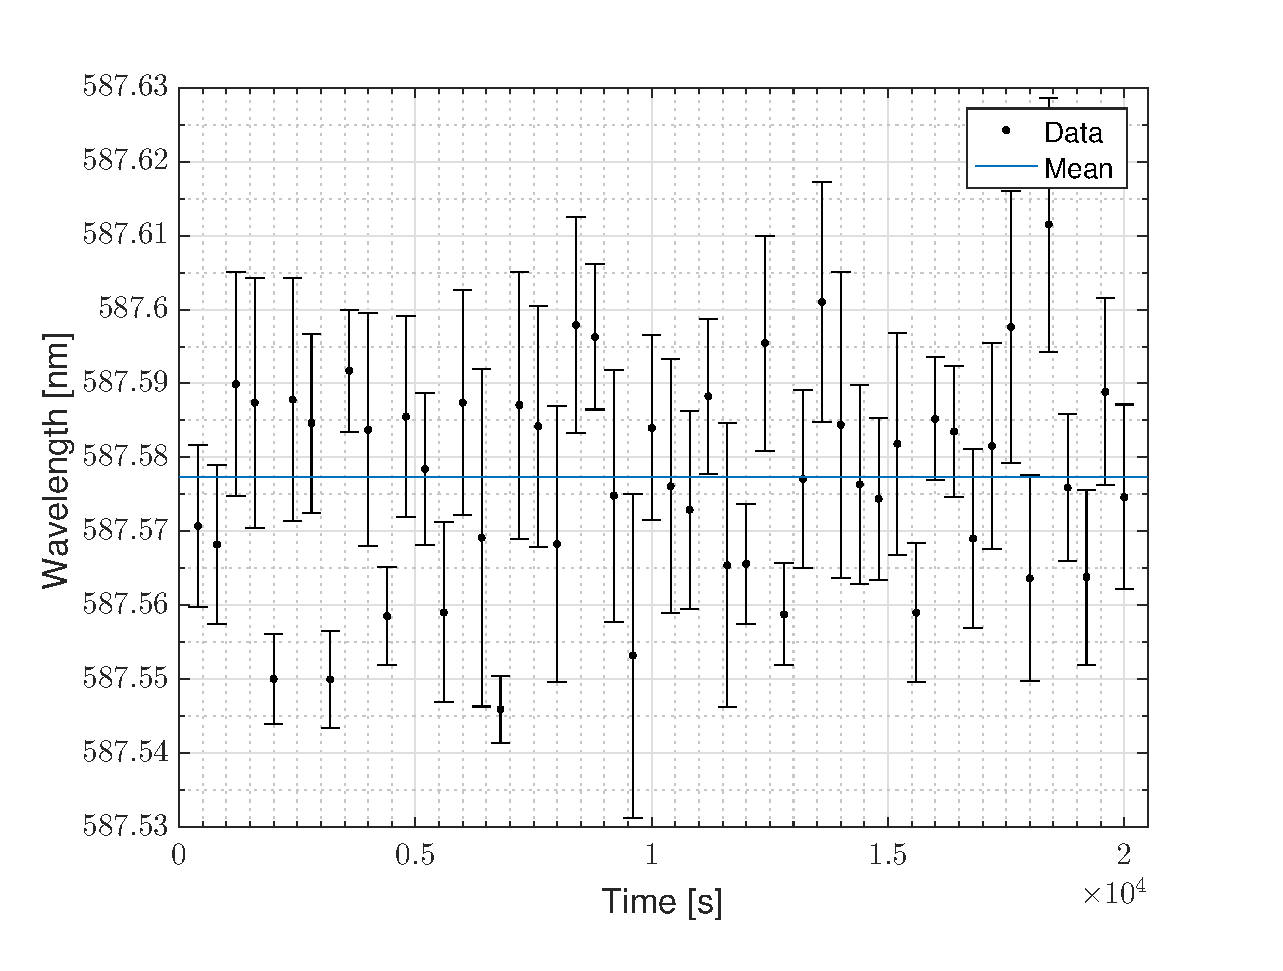
\includegraphics[width = .7\linewidth]{vib_587_bins_med_usikkerhed.eps}
\caption{Wavelengths measured with bins containing twenty measurements for peak 4.}
\label{fig: exp2 bins}
\end{subfigure}
~
\begin{subfigure}{0.9\textwidth}
\centering
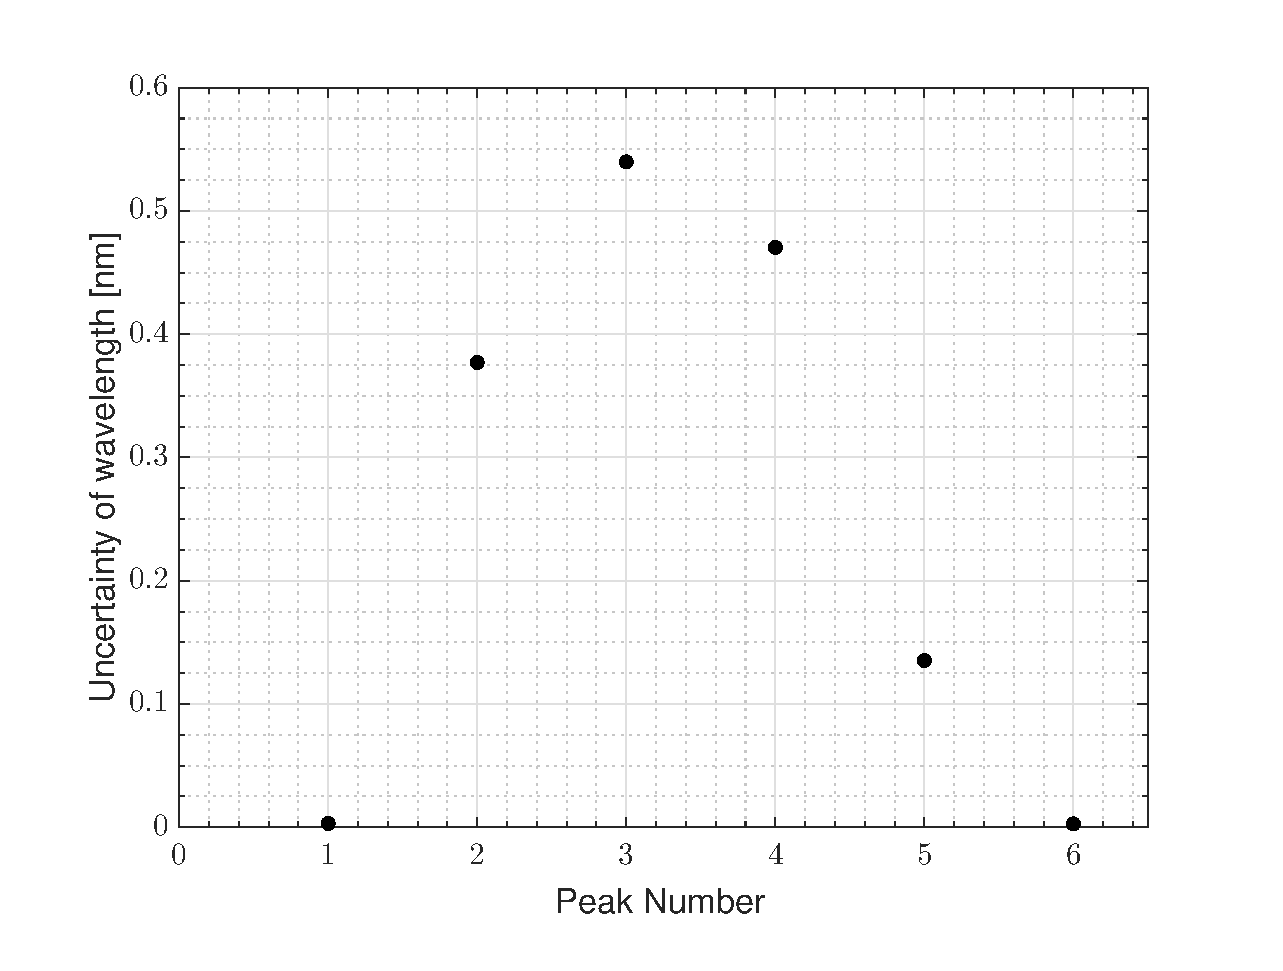
\includegraphics[width = .7\linewidth]{vib_usikkerhed_alle.eps}
\caption{The uncertainty of the average wavelength for every peak.}
\label{fig: exp2 usikkerhed peaks}
\end{subfigure}
\caption{In the top panel the calculated average wavelengths for peak 4, when stacking twenty measurements, are shown over time. The uncertainty of each wavelength is illustrated with errorbars and the mean over all the found wavelengths is shown. In the bottom panel the uncertainty of the total average wavelength found for each peak is shown.}
\label{fig: exp2 samlet bins}
\end{figure}

\newpage
\section{Third Experiment - Temperature Variations}

For the third experiment, 60 measurement were made for twelve different temperature steps. The temperatures are listen in Tbl. \ref{tbl: temp}.

\begin{table}[!h]
\centering
    \begin{tabular}{cccccc}
    \hline
    Step & Temperature [°C] & Step& Temperature [°C] & Step  & Temperature [°C] \\
    \hline
    1    & 19.5             & 5 & 32.4             & 9  & 42.2             \\
    2    & 25.0             & 6 & 35.9             & 10 & 44.8             \\
    3    & 28.1             & 7 & 36.9             & 11 & 47.8             \\
    4    & 29.9             & 8 & 39.8             & 12 & 49.3             \\
    \hline
    \end{tabular}
    \caption{The twelve temperature steps at which measurements were made for the third experiment.}
    \label{tbl: temp}
\end{table}


In the 60 measurements the six peaks were fitted in the same way as in the first and second experiment. The wavelengths measured for each peak in the 60 measurements were then used to calculate the average wavelength for every peak and their uncertainties were calculated. This was done for all temperatures. The measured shifts in wavelengths induced by the change in temperature for all six peaks are shown in Fig. \ref{fig: exp3 1_6}. 

\begin{figure}[!h]
\centering
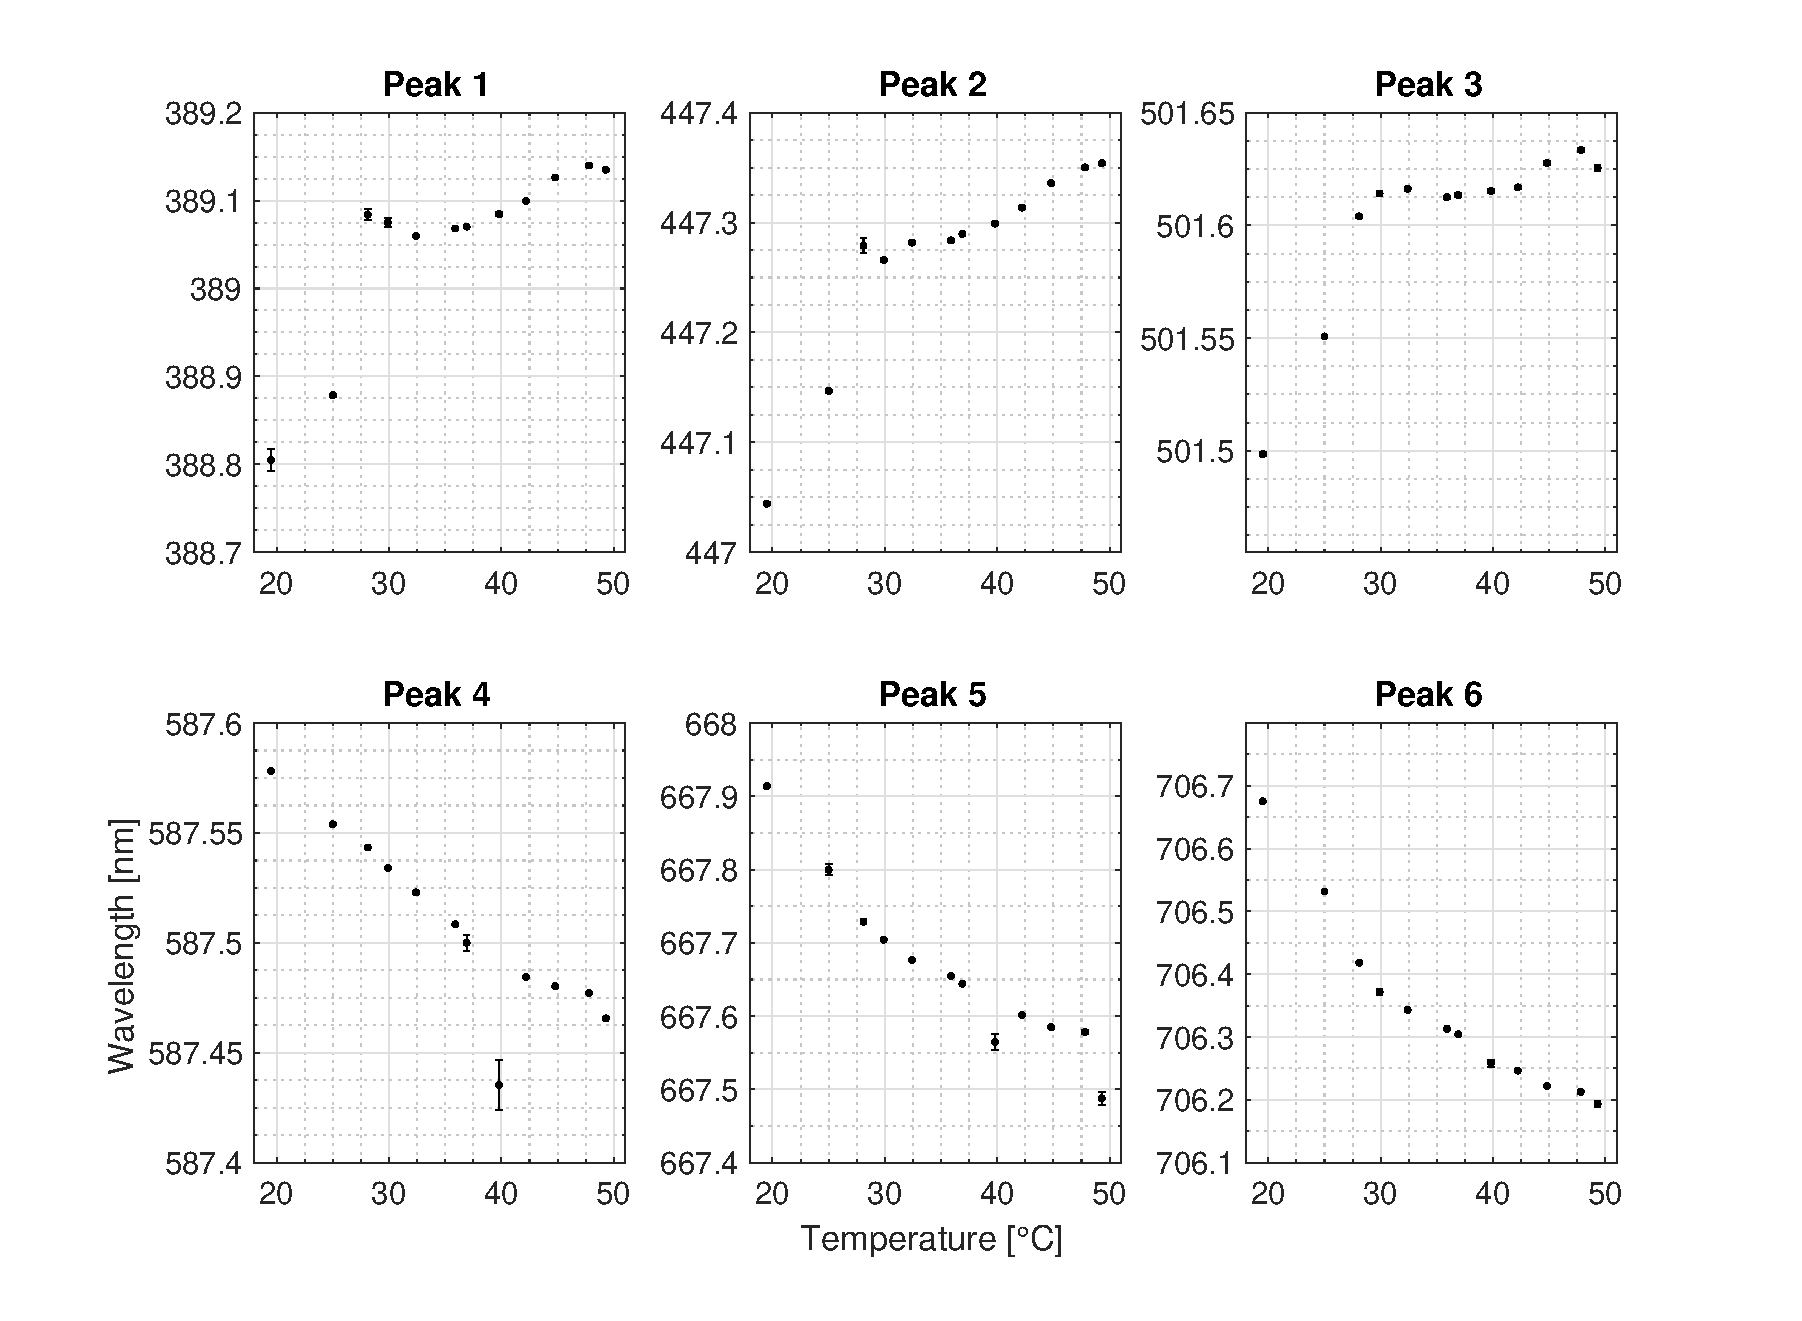
\includegraphics[width=\textwidth]{1_6_temp.eps}
\caption{The measured wavelengths by the spectrograph, for the six emission lines as a function of temperature. Uncertainties are calculated with Eq. \ref{eq: Sx}.}
\label{fig: exp3 1_6}
\end{figure}

Under the assumption, that the measured wavelengths of the peaks are shifted linearly as a function of temperature, the shift in wavelength for each peak  as a function of temperature was fitted to the function,
\begin{align}
\lambda_{shift}(T) = a_{shift} T + \lambda_{Laboratory}, 
\end{align}
where $\lambda_{shift}$ is the shifted wavelength value, $a_{shift}$ is the shift in wavelength per °C, $ T$ is the temperature and $\lambda_{Laboratory}$ is the the laboratory wavelength. The uncertainties, in form of the standard deviation, for the slope coefficients were found from their 95\%-confidence interval. 
\\
Based on the results in Fig. \ref{fig: exp3 1_6}, the slope coefficients, $a_{shift}$, for the six peaks were plotted against the wavelengths of the peaks. The slope coefficients as a function of wavelength were then fitted to the function,
\begin{align}
a_{shift}(\lambda) =  a_{slope} \lambda + b_{offset}, 
\label{eq: slope}
\end{align}
where $a_{slope}$ is the change of the $a_{shift}$ coefficients per wavelength, $\lambda$, and $b_{offset}$ is an offset.

The $a_{shift}$ coefficients as a function of wavelength are shown together with the fitted Eq. \ref{eq: slope} in Fig. \ref{fig: exp3 slope coeff.}.

\begin{figure}[!h]
\centering
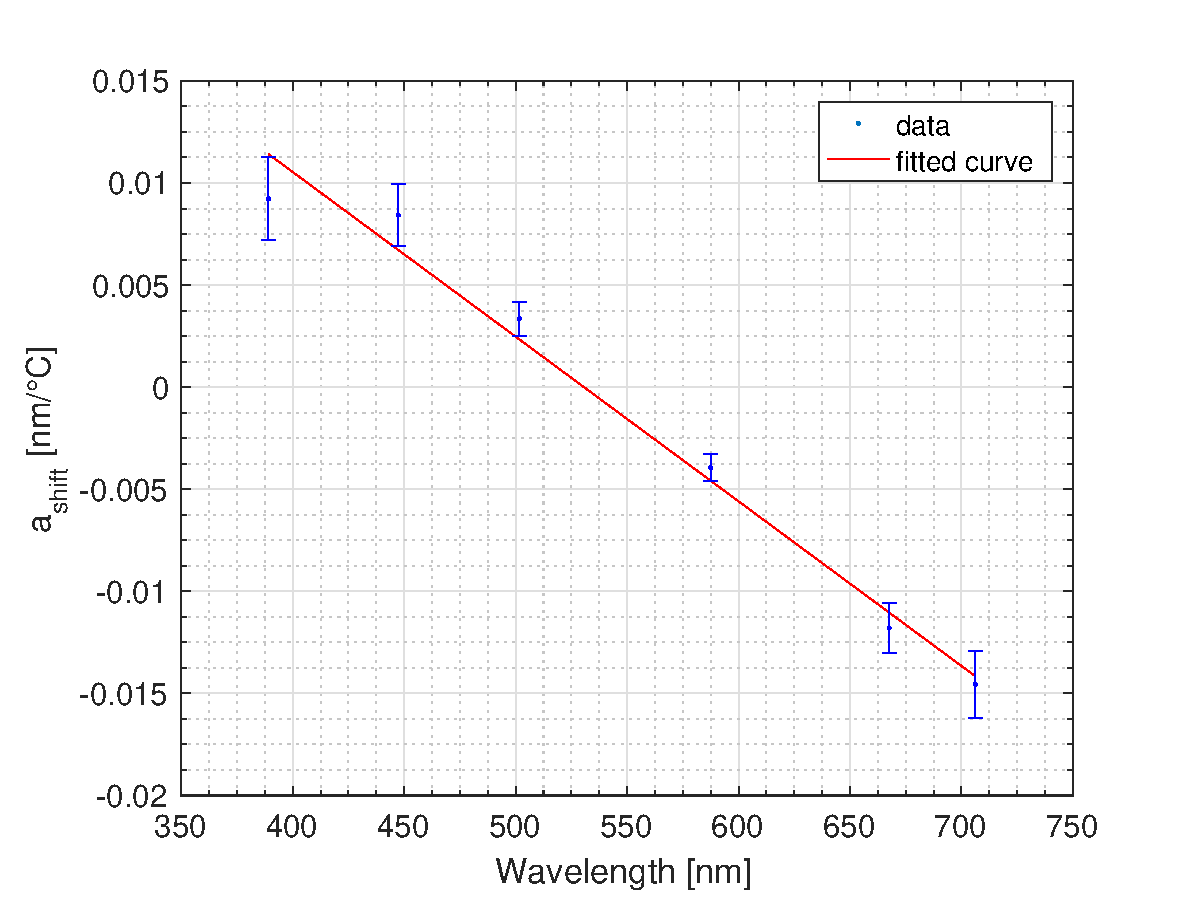
\includegraphics[width = \textwidth]{slope_function_of_wavelength.eps}
\caption{The $a_{shift}$ coefficients are shown as function of wavelength. The $a_{shift}$ coefficients are found by a linear fit to the measured wavelengths, for every emission line, under the assumption, that the found wavelengths of the peaks are shifted linearly as a function of temperature.}
\label{fig: exp3 slope coeff.}
\end{figure}

The results from the three experiments will be discussed in the following chapter.






\chapter{Discussion}

The three developed experiments were to simulate the conditions the spectrograph would be exposed to if it were placed in space. 

The first experiment took measurements over a long period of time with the spectrograph being stationary. The results from the first experiment, showed that using a single measurement from the spectrograph meant that the uncertainties of the found wavelengths were of the order of \SI{1}{\nano\meter}. Further analysis of the data showed that binning measurements together and averaging their values, meant that the wavelengths could be identified with uncertainties of the order of \SI{d-3}{\nano\meter}. The use of multiple measurements is a method already used to average the cosmic rays producing additional counts in pixels on the CCD \citep{Mons}. Stacking of measurements to determine the wavelength was therefor used in the following two experiments. 

It was clear from the first experiment that it would be ideal to do further tests of the spectrograph to investigate the cause of the "shoulder" peak in the measurements, shown in fig. \ref{fig: double gauss}. To determine the cause of this, the spectrograph would have to bee taken apart for further examination which was beyond the scope of this thesis. It would be ideal to run the experiments again once the cause of the "shoulder" peak has been identified and removed. 
The final results of the first experiment suggested that the wavelength midrange has the largest stability in determining the wavelengths of the emission lines, corresponding to a smaller uncertainty of the found wavelength as shown in fig. \ref{fig: exp1 usikkerhed peaks}. This was expected as the strongest emission line was located in this range. The order of the uncertainty was also expected to be in the found range as the resolution of the spectrograph was \SI{0.01}{nm}.
\\
\\
For the second experiment the precision of the wavelengths measured for the six peaks was examined under simulation of jitter due to pointing of the satellite. The measurements were binned and an average wavelength was found for each peak. The results of the second experiment found that the wavelengths for the peaks were measured with larger uncertainties than in the first experiment. Opposite the first experiment, the second experiment suggests that the stability of the wavelengths measured for the peaks is smallest in the midrange of the spectrograph. This was not the expected result for the second experiment. It was expected that the uncertainties would be of a larger order due to the movement of the spectrograph, causing the light to hit the slit from different angles. It was, however, also expected that the wavelength midrange would be the must stable, which turned out to not be the case. The reason for the change of the most stable range compared to the first experiment is not known.
This indicates the need for the experiment to be run again to see if the results can be reproduced before concluding on the final results. 
\\
\\
The third experiment examined the shift in measured wavelengths for the six peaks as a function of temperature. For peak 1 to peak 3, which cover the range from \SI{388}{\nano\meter} to \SI{503}{\nano\meter}, the results shown in fig. \ref{fig: exp3 1_6} showed that peaks were shifted to higher wavelengths. The results also indicated that the wavelength shifts for peak 1 to 3 decreased with increasing wavelength.
\\
For peak 4 to 6, which cover the range from \SI{587}{\nano\meter} to \SI{706}{\nano\meter}, the results showed that the peaks were shifted to lower wavelengths. The shift to lower wavelength increased for the peaks going from peak 4 to 6. 
\\
\\
Furthermore from the results it seemed that the shifts for the peaks 4 to 6, were linearly dependent of temperature. For peak 1 to 3 it was not clear that the shifts were linearly dependent on temperature, as the measurements around \SI{30}{\degreeCelsius} were outliers for this to be the case. However, based on the results for peak 4 to 6, the assumption that the shifts for all peaks were linear dependent of temperature was made. The identified wavelength for each peak was then fitted to a linear function of the temperature, so the slope for each fit could be compared. This was done in fig. \ref{fig: exp3 slope coeff.} which suggested that the slopes for the different fits were themselves linear dependent of the wavelength. It was expected that the measured wavelengths were dependent on the temperature, but the fact that the shift as a function of temperature was not the same for all the emission lines was not expected. The cause of the none uniform shift over the wavelength range is expected to lay within the spectrograph, but pinpointing the exact cause is not possible without taking the spectrograph apart and conducting further experiments.
For the results of the third experiment to be verified, the experiment would need to be run several times again and produce similar results before being able to conclude that they are in fact correct. Especially the assumption that the wavelength shifts for all the emission lines are linearly dependent of temperature, would need to be verified by further experiments.

The experiments designed to test the spectrograph have shown that the experiment to be done from this point forward, would include taking it apart to examine what is happening inside during the experiments, especially during the second and third experiment. 



\chapter{Conclusion}
In this thesis the USB4000 spectrograph was examined to illuminate the possibilities and limitations for using a compact spectrograph for observations in space onboard a Cubesat. Taking in to consideration the environment satellites are subject to, three experiments were developed and build to test the measurements from the spectrograph, on six of the emission lines of Helium. 
\\
\\
The first experiment examined the stability of stationary measurements over a long period of time. From the first experiment it was found that noise in form of "shoulder" peaks was present at a constant distance from the true peaks in the measured spectra. It was found that the noise from the "shoulder" peaks could be filtered out in the analysis so the wavelengths for the true peaks could be measured with the uncertainties in the range \SIrange{0.1d-3}{1.1d-3}{\nano\meter}.

In the second experiment the stability of measurements when simulating pointing of the satellite, by vibrations was examined. It was measured that with simulated pointing the wavelengths of the lines could be measured with uncertainties in the range \SIrange{0,01}{0,54}{\nano\meter}.

The third experiment tested the effect on the measurements taken when the temperature was varied. It was measured that the wavelength of the peaks were shifted when the temperature was varied for the measurements, but the cause of the shift was not found. The results from the third experiment showed that the shifts of the six peaks were not identical. A theory was suggested that the rate of change of wavelength for the different peaks was linearly dependent of wavelength however it was concluded that further experiments must be conducted with similar results in order to verify this theory.


%%%%% BIBLIOGRAPHY %%%%%
\nocite{*}
\bibliographystyle{plainnat}
\bibliography{references}
\end{document}
